\documentclass[../thesis/thesis.tex]{subfiles}
\begin{document}

\chapter{Design}
\label{chap:design}

In this chapter, we describe the methodology used to design our \gls{vc} investment screening system. Figure~\ref{fig:design:system_architecture} depicts the architecture of our system, structured into five components: data collection, dataset preparation, pipeline creation, pipeline selection, and prediction. We evaluate the performance of this system in the next chapter.

\begin{figure}[!htb]
    \centering
    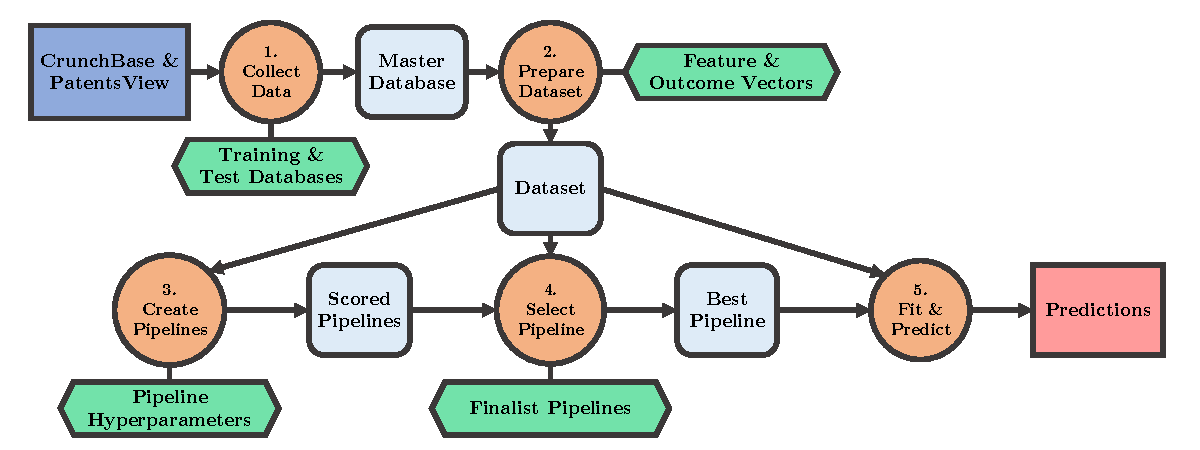
\includegraphics[width=\textwidth]{../figures/design/flowchart_overview}
    \caption[System architecture flowchart]{An overview of the system architecture proposed by this project. Legend: dark blue square~=~input, orange circle~=~system component, light blue rounded square~=~intermediate, red square~=~output, green hexagon: iterative process / search space.}
    \label{fig:design:system_architecture}
\end{figure}

\begin{enumerate}

\item Data Collection. We developed a conceptual framework to guide our feature and data source selection. Based on this framework, we decided to collect data from CrunchBase and PatentsView. Our system collects data from these sources and imports it into a relational database.

\item  Dataset Preparation. The system extracts database slices and converts them into datasets suitable for supervised learning. The system cleans the databases to ensure they only include relevant companies. We report the descriptive statistics of an indicative dataset.

\item Pipeline Creation. We identified issues of sparsity, long-tailed distributions, imbalanced feature ranges, and non-orthogonality in our datasets. We developed a classification pipeline system to address these dataset issues. Our system performs a grid search across the hyperparameters of the pipeline to generate scored, candidate pipelines.

\item Pipeline Selection. Next, our system selects the best candidate pipelines and evaluates their robustness over time. The outcome of this process is a single pipeline optimised to suit the dataset and prediction task. To evaluate robustness over time, we recreated historical datasets using a technique that filters records by their time-stamps.

\item Model Fit and Prediction. Finally, our system applies the optimised pipeline to a feature vector from a held-out test database, which generates a model and a set of predictions. We evaluate the models and predictions produced by our system in the next chapter.

\end{enumerate}

\section{Data Collection}

In the previous chapter, we reviewed features and data sources used in entrepreneurship and \gls{vc} investment research. In this section, we first discuss how we developed a conceptual framework to guide our feature and data source selection and then describe the process of collecting and storing data from CrunchBase and PatentsView.

\subsection{Conceptual Framework}

While previous studies into startup performance have explored a range of features, few individual studies have evaluated a comprehensive and diverse feature set. We developed a conceptual framework to ensure we included a comprehensive set of features in our \gls{vc} investment screening system.

Our conceptual framework built on previous work by Ahlers (2015) to model investment decisions on equity crowd-funding platforms~\cite{ahlers2015}. We sought to generalise Ahlers' framework beyond equity crowd-funding. While the first factor of their framework (venture quality) applies to startups generally, they defined their second factor (investment confidence) with respect to features specific to equity crowd-funding. We developed this second factor further, describing investment confidence as a product of third party validation, historical performance and contextual cues.

Our proposed conceptual framework is depicted in Figure~\ref{fig:design:features:framework_details}. In the previous chapter, we described the features that underpin each factor and outlined the theoretical and empirical evidence that justify their inclusion in our conceptual framework.

\begin{figure}[!htb]
    \centering
    
\begin{forest}
    forked edges,
    for tree={
        grow=west,
        l sep = 1cm,
        fork sep = 0.5cm,
        align=center,
        tier/.pgfmath=level(),
        child anchor=east,
        anchor=base east,
        edge={<-, thick},
        every node={rectangle,draw=black}
    }
[Startup\\Investment,
    [Startup\\Potential,
        [Human\\Capital,
            [Founder Capabilities]
            [Advisor Capabilities]
            [Executive Capabilities]
        ]
        [Social\\Capital,
            [Social Media]
            [Events Influence]
            [Strategic Alliances]
        ]
        [Structural\\Capital,
            [Patent Filings]
        ]
    ]
    [Investment\\Confidence,
        [Third Party\\Validation,
            [Investment Record]
            [Investor Reputation]
            [Media Coverage]
        ]
        [Historical\\Performance,
            [Financial Performance]
            [Non-Financial Performance]
        ]
        [Contextual\\Cues,
            [Industry Performance]
            [Local Economy]
            [Broader Economy]
        ]
    ]
]
\end{forest}

    \caption[Conceptual framework for \gls{vc} investment.]{Proposed conceptual framework for \gls{vc} investment. We adapted the framework proposed by Ahlers et al.~\cite{ahlers2015}, originally based on work by Baum and Silverman~\cite{baum2004}. This framework includes features identified by the literature review in Chapter~\ref{chap:litreview}.}
    \label{fig:design:features:framework_details}
\end{figure}

\subsection{Data Sources}

We sought data sources that could provide features that support the factors in our conceptual framework. We decided to collect data from CrunchBase with supplementation from PatentsView, a patent filings database. These sources cover the majority of factors in our conceptual framework. We discuss the process of collecting data from these sources, as depicted in Figure~\ref{fig:design:data_collection}.

\begin{figure}[!htb]
    \centering
    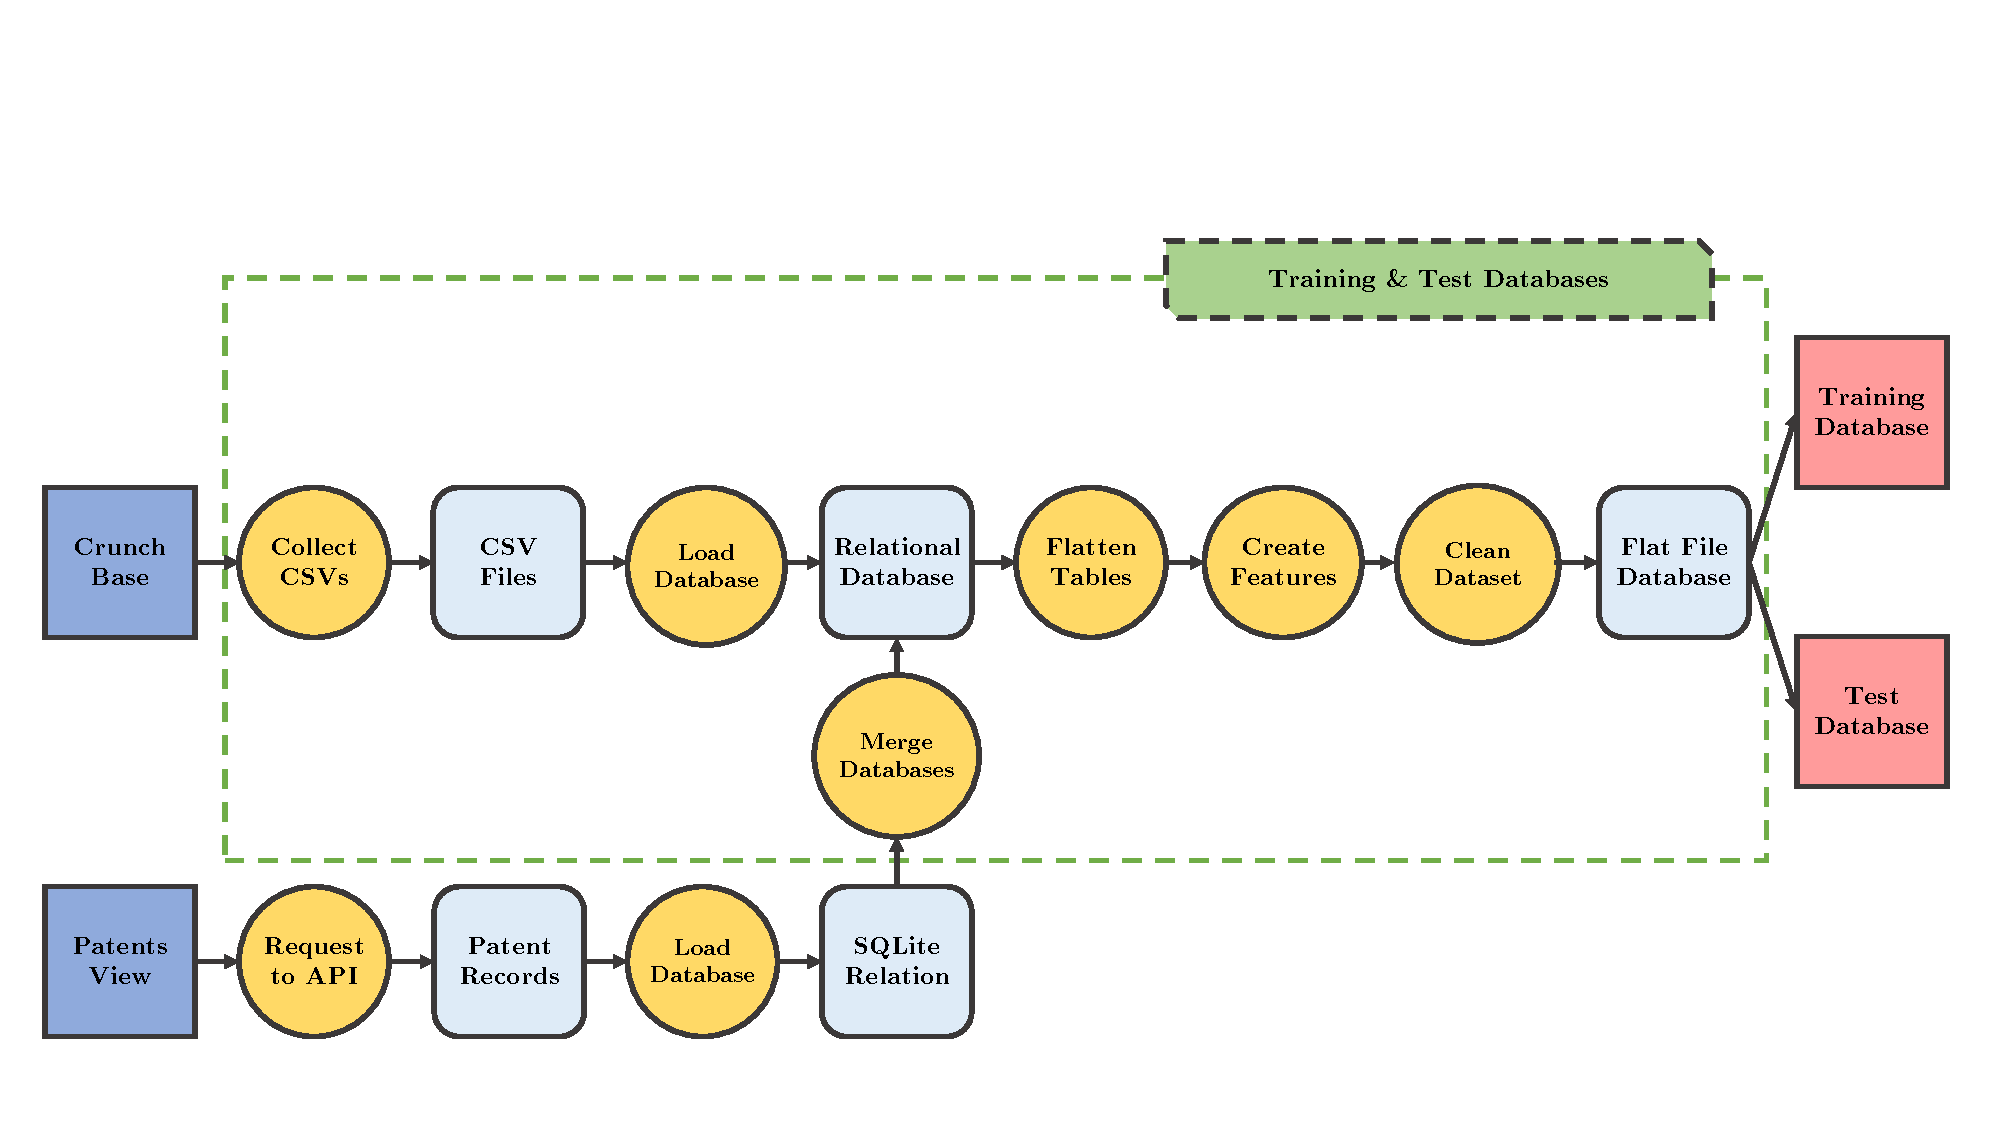
\includegraphics[width=\textwidth]{../figures/design/flowchart_data_collection}
    \caption[Data collection flowchart]{Data collection overview. CrunchBase data is collected multiple times to produce separate training and testing databases. Legend: dark blue square~=~input, yellow circle~=~process, light blue rounded square~=~intermediate, red square~=~output, green hexagon: iterative process / search space.}
    \label{fig:design:data_collection}
\end{figure}

\subsubsection{CrunchBase}

We were granted an Academic License to collect data from CrunchBase. CrunchBase provides database access in a few formats that offer trade-offs in terms of accessibility and comprehensiveness: REST API, CSV Dumps, MS Excel Summary. We chose to use the CSV Dumps because they provided a good trade-off between ease of use and comprehensiveness of access. CrunchBase provides a CSV file for each of CrunchBase's primary endpoints (e.g. organisations, people, funding rounds) which can be loaded easily into relational databases (see Appendix~\ref{appendix:database_schema} for the database schema). We downloaded CSV Dumps from CrunchBase on 09 September 2016 and 04 April 2017 which became our training and testing databases, respectively.

\subsubsection{PatentsView}

We used PatentsView to obtain the patent filing records of each company in our CrunchBase dataset, focusing on information relating to dates, citations, and patent types. Our system matches companies across CrunchBase and PatentsView by standardising the company names (removing common suffixes, punctuation, etc.) and using normalised Levenshtein distances to determine similarity. Although approximate matching introduces error, the volume of companies in the database is too high to be matched manually, and there are no other identifying records. We stored the PatentsView data in a relation which we merged into our CrunchBase data to form our master databases.

\section{Dataset Preparation}

Our system performs multiple steps to prepare datasets from our training and test databases for use in machine learning, as depicted in Figure~\ref{fig:design:dataset_preparation}. In this section, we describe the process of preparing our datasets, which involves two components: generating historical databases from our relational database and converting these relational database slices into clean datasets ready for machine learning. Finally, we present the descriptive statistics of our dataset.

\begin{figure}[!htb]
    \centering
    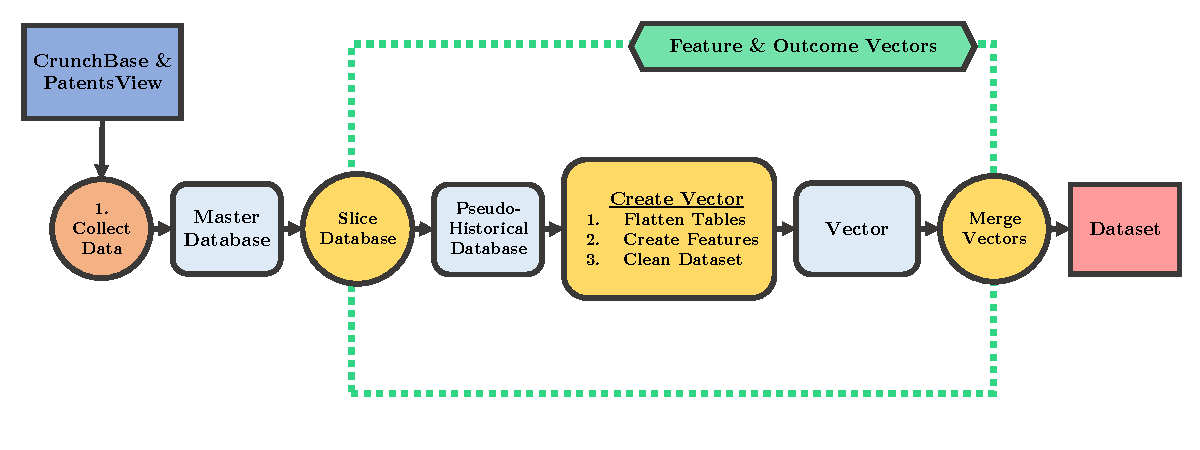
\includegraphics[width=\textwidth]{../figures/design/flowchart_dataset_preparation}
    \caption[Dataset preparation flowchart]{Dataset preparation overview. Feature and outcome vectors are created from the master relational database. Legend: dark blue square~=~input, yellow circle~=~process, light blue rounded square~=~intermediate, red square~=~output, green hexagon: iterative process / search space.}
    \label{fig:design:dataset_preparation}
\end{figure}

\subsection{Database Slicing}

We developed a procedure for generating historical databases from our CrunchBase and PatentsView data. CrunchBase provides `created-at' and `last-updated' time-stamps for each record in their CSV-formatted dumps (and also in the JSON-formatted responses from their API). We used this to reverse-engineer previous database states by filtering the master database to only include records created before a given `slice' date.

We evaluated our slicing technique by comparing a CrunchBase database collected in December 2013 with a slice engineered from our training database (collected in September 2016), as shown in Figure~\ref{fig:design:counts_slice_method}. There are only minor differences in the counts between the methods.

\begin{figure}[!htb]
    \centering
    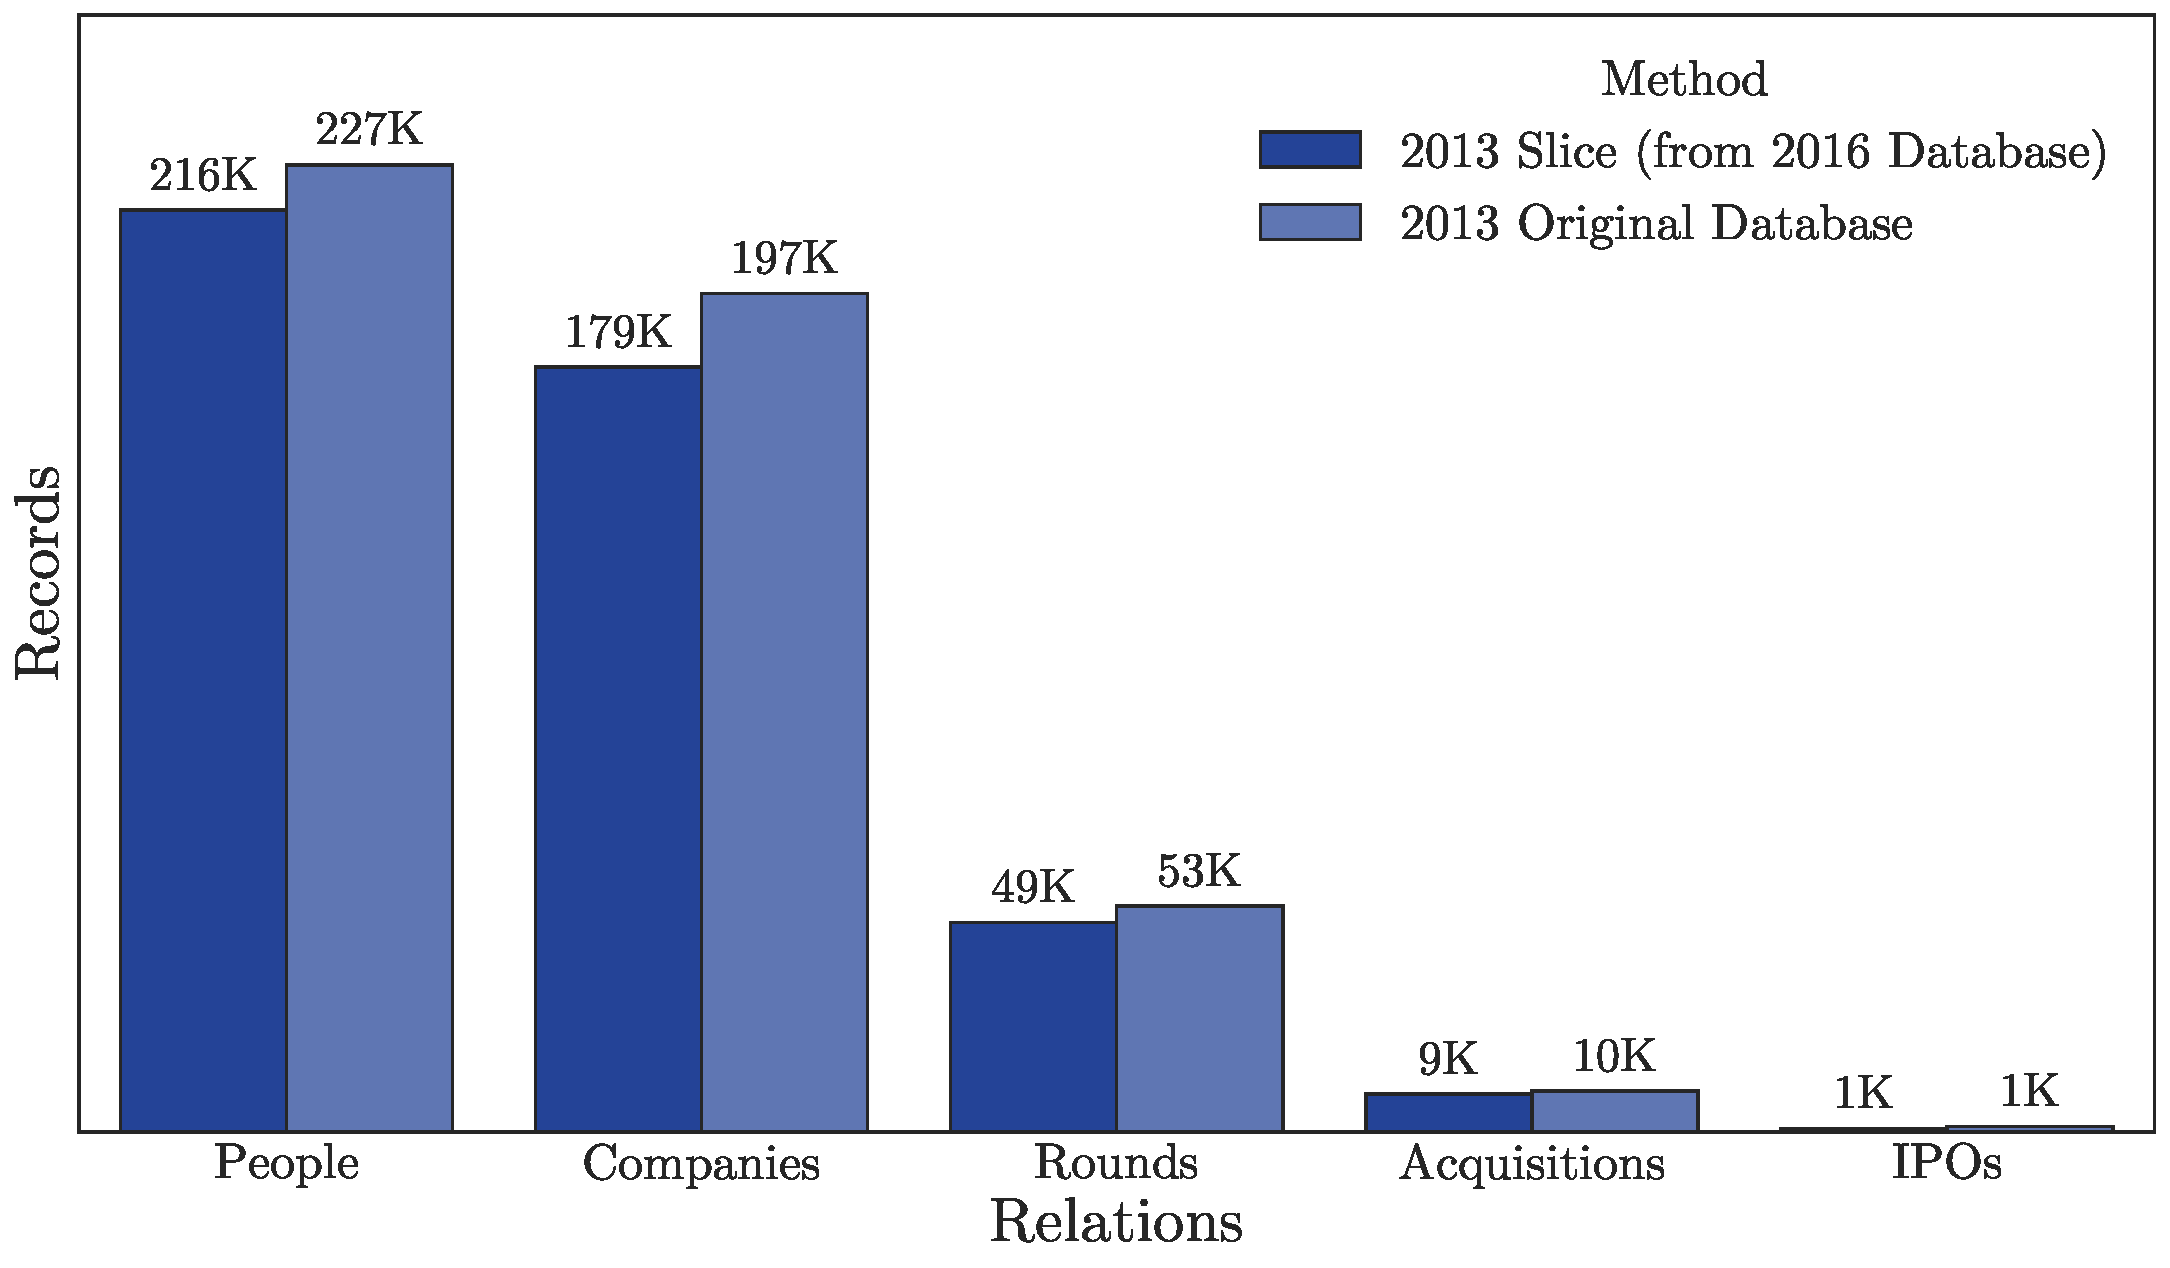
\includegraphics[width=\textwidth]{../figures/design/counts_slice_method}
    \caption[Database slice compared with original database]{Database slice compared with original database. Original database collected in December 2013. Database slice generated from the training database collected in September 2016 and sliced to only include records created prior to December 2013.}
    \label{fig:design:counts_slice_method}
\end{figure}

Figure~\ref{fig:design:slice_counts_over_time} presents company counts by startup development stage from different dataset slices. Dataset counts across all developmental stages have steadily increased over time. Before 2012 the datasets become too small to use to make meaningful predictions.

\begin{figure}[!htb]
    \centering
    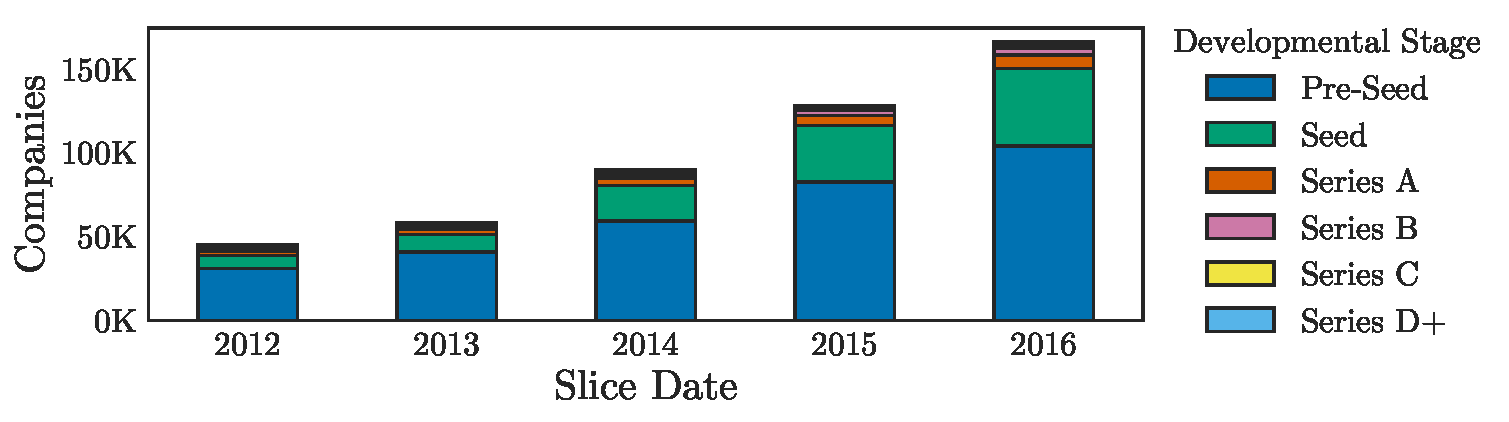
\includegraphics[width=\textwidth]{../figures/design/counts_stage_slice}
    \caption[Dataset counts over time]{Dataset slice counts over time. Each slice was generated on April 04 of each respective year. Proportions by developmental stage stay relatively constant over this time-frame.}
    \label{fig:design:slice_counts_over_time}
\end{figure}

\subsection{Vector Creation}

To prepare our datasets for machine learning, our system performs aggregation, feature creation and preliminary screening. In the following section, we evaluate the effect of these processes on an indicative database sliced from the training database as of 09 September 2016 (N~=~425,934).

First, our system flattens the relational database slices into a single file using \gls{sql} aggregation queries. The system aggregates each relation in turn, grouping by Company ID and combining each aggregated table using left outer joins. Next, the system converts tuples (e.g. Round Type and Round Date) and lists (e.g. Round Types) into dummy variables.

Our system performs preliminary screening to remove traditional, non-startup businesses from the dataset (e.g. consulting firms, companies that will not take \gls{vc} funding, etc.). To do this, we explored two factors for each company: developmental stage and age. By developmental stage, we primarily refer to external funding milestones. These stages also indicate shifts in a startup's functions and objectives. Our dataset as grouped by startup developmental stage is depicted in Figure~\ref{fig:design:lifecycle}.

\begin{figure}[!htb]
    \centering
    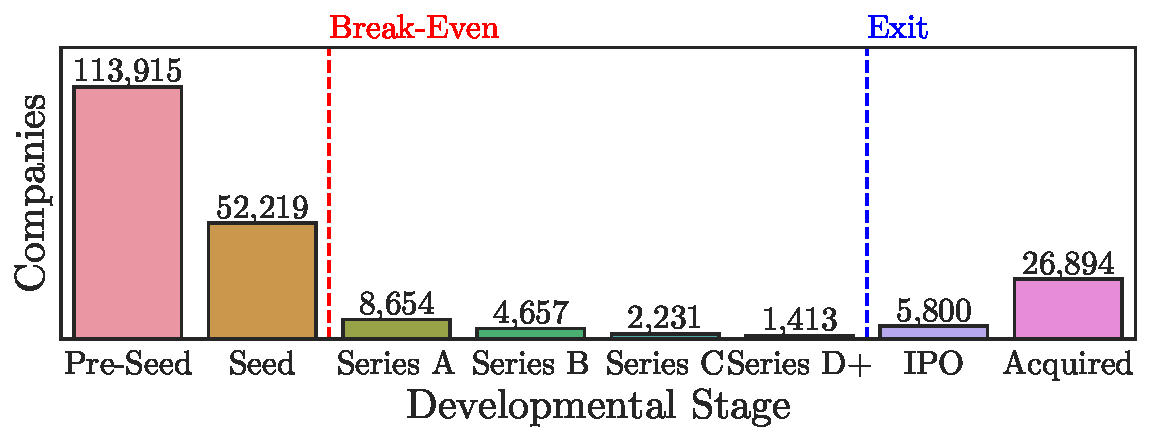
\includegraphics[width=\textwidth]{../figures/design/descriptives_counts_stage}
    \caption[Startup development life-cycle]{Companies grouped by stages of the startup development life-cycle. Companies at Pre-Seed and Seed stages are typically unprofitable and seek external funding to sustain their operations. Companies at Series A - Series D+ are typically either profitable or at least revenue-generating, and seek external funding to expand their operations.}
    \label{fig:design:lifecycle}
\end{figure}

After attempting to place the companies into development stages, a large group of companies that have not raised funding remain. We classify these companies into two groups -- those that intend to raise funding and those that do not. We applied a cut-off equal to the 90th percentile of the age of companies in the Seed category and excluded the older group from further analyses (N~=~227,162,  53.3\%). As we are only interested in companies that could seek investment, we also excluded Closed, Acquired and IPO groups from further analyses (N~=~35,973, 8.4\%).

Figure~\ref{fig:design:stages_ages} depicts the ages of companies in the dataset grouped by developmental stage. There is a positive relationship between age and developmental stage. Most pre-Series A companies are under five years old, and the majority of Series D+ funded companies are under ten years old, and the 75th percentile is at 15 years old. On this basis, we excluded companies that are over the 75th percentile for the age of companies in the Series D+ category (N =9,756, 2.2\%). Our preliminary screening reduced the dataset from 425,934 companies to 153,043 companies, a reduction of 64.1\%.

\begin{figure}[!htb]
    \centering
    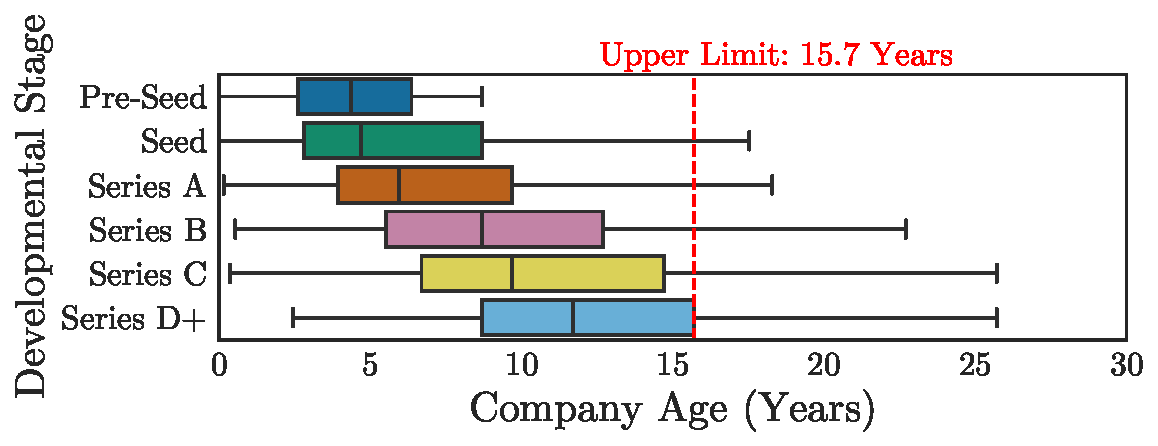
\includegraphics[width=\textwidth]{../figures/design/descriptives_ages_stage}
    \caption[Company ages by developmental stage]{Company ages in years grouped by developmental stage. The dashed red line represents the 75th percentile of the age of companies in the Series D+ category (15.7 years).}
    \label{fig:design:stages_ages}
\end{figure}

\subsection{Descriptive Statistics}

Table~\ref{tab:design:descriptive_statistics} presents the descriptive statistics for the cleaned dataset from the previous section. The dataset skews towards Pre-Seed companies (i.e. companies that were recently founded and had not raised funding yet, 68.9\%). These companies have few available features in comparison to later developmental stages. We investigate the impact of this on our predictions in Chapter~\ref{chap:evaluation}. The interquartile ranges imply significant variability in all measures. We do not believe that this indicates that the data has not been cleaned adequately, but rather, that it reflects that startup companies vary in their traits.

\begin{table}[!htb]
    \centering
    \scalebox{0.9}{\begin{tabular}{lrrrrrrrrrrr}
\toprule
Stage &	Obs &
\multicolumn{2}{c}{\thead{Age\\(Years)}} &
\multicolumn{2}{c}{\thead{Funding Raised\\(USD, M)}}	&
\multicolumn{2}{c}{\thead{Funding\\Rounds (N)}}	&
\multicolumn{2}{c}{\thead{Patent\\Filings (N)}}	&
\multicolumn{2}{c}{\thead{Available\\Features (N)}}	\\
{}          & N         & 50th  & 75th  & 50th  & 75th  & 50th  & 75th  & 75th  & 90th  & 50th  & 75th \\ \midrule
Pre-Seed    & 113,915   & 4.36  & 6.36  & 0.00  & 0.00  & 0     & 0     & 0     & 0     & 25    & 133 \\
Seed        & 38,942    & 4.66  & 6.69  & 0.25  & 1.30  & 1     & 2     & 0     & 1     & 178   & 231 \\
Series A    & 6,615     & 5.69  & 8.70  & 4.40  & 9.41  & 2     & 3     & 0     & 2     & 239   & 302 \\
Series B    & 3,342     & 7.61  & 10.70 & 14.89 & 28.20 & 3     & 4     & 0     & 4     & 255   & 314 \\
Series C    & 1,610     & 8.70  & 11.70 & 35.29 & 62.00 & 3     & 5     & 1     & 9     & 305   & 321 \\
Series D+   & 998       & 9.70  & 12.70 & 74.39 & 130.8 & 5     & 7     & 4     & 19    & 319   & 330 \\
Included    & 165,422   & 4.69  & 6.69  & 0.00  & 4.00  & 1     & 2     & 0     & 1     & 90    & 160 \\
\bottomrule
\end{tabular}
}
    \caption[Descriptive statistics by developmental stage]{Descriptive statistics grouped by developmental stage.}
    \label{tab:design:descriptive_statistics}
\end{table}

CrunchBase's industry classification is simplistic compared to other databases (e.g. USSIC, VentureSource) which take a structured, hierarchical approach. For example, ``Software'', ``Internet Services'' could describe the majority of companies included in the database and account for 16.4\% and 13.4\% of all companies in the dataset respectively (see Figure~\ref{fig:design:industry_counts}). Despite these vague labels, it is evident the dataset skews towards high technology startups, as opposed to biomedical, agricultural, or other technologies (which do not make the Top 10).

\begin{figure}[!htb]
    \centering
    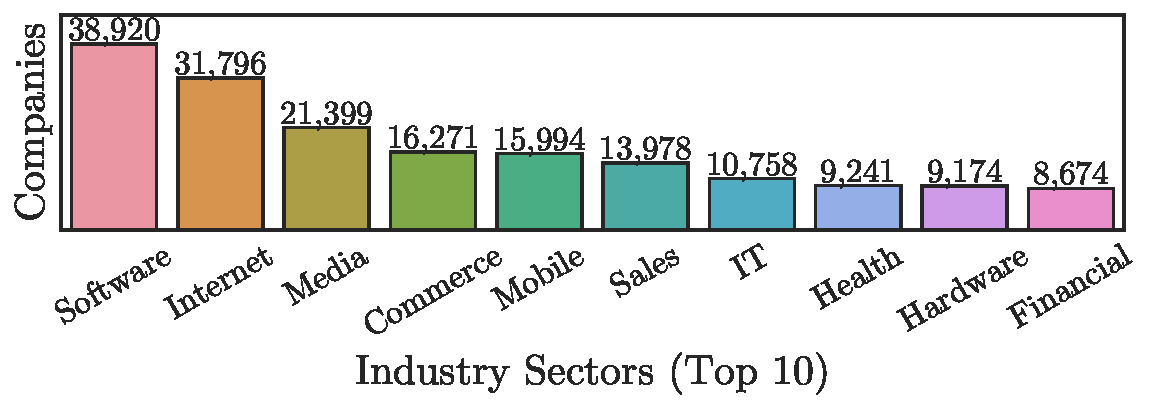
\includegraphics[width=\textwidth]{../figures/design/descriptives_counts_industry}
    \caption[Company counts by industry sector]{Companies grouped by industry sector. Industry labels are not mutually-exclusive. The 10 most common sectors are displayed.}
    \label{fig:design:industry_counts}
\end{figure}

\section{Pipeline Creation}

In the following section, we perform exploratory data analysis on our dataset and decide that a classification pipeline system could help us to address issues identified. The classification pipeline system is depicted in Figure~\ref{fig:design:pipeline_creation}.

\begin{figure}[!htb]
    \centering
    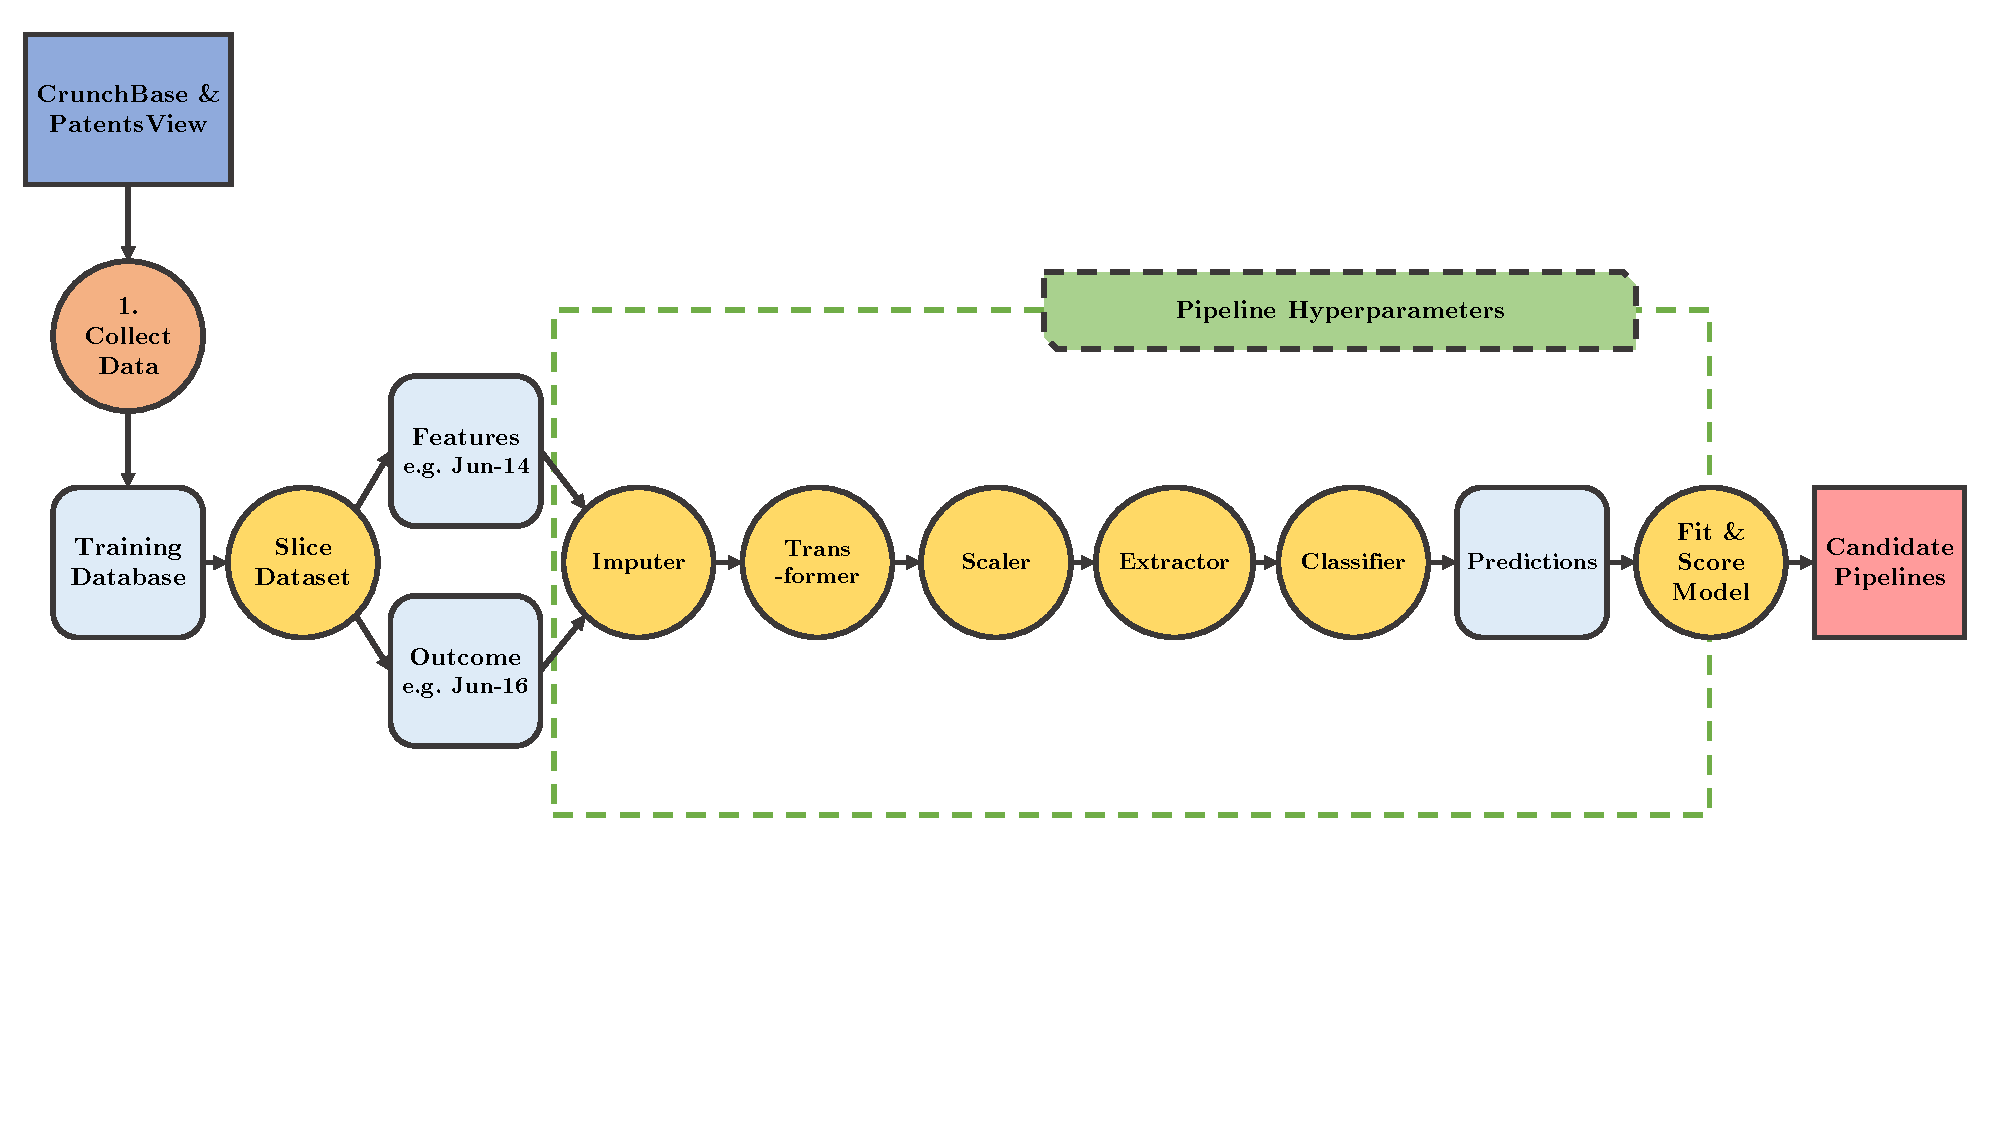
\includegraphics[width=\textwidth]{../figures/design/flowchart_pipeline_creation}
    \caption[Pipeline creation flowchart]{Pipeline creation overview. Grid search is performed across the pipeline hyperparameters to generate a variety of scored, candidate pipelines. Legend: dark blue square~=~input, orange circle~=~system component, yellow circle~=~process, light blue rounded square~=~intermediate, red square~=~output, green hexagon: iterative process / search space.}
    \label{fig:design:pipeline_creation}
\end{figure}

\subsection{Exploratory Analysis}

We performed exploratory data analysis on our dataset to assess what techniques would be suitable and the need for any further pre-processing. We identified dataset issues that include sparsity, long-tailed distributions, imbalanced feature ranges, and non-orthogonality.

\subsubsection{Sparsity}

We explored the sparsity of the dataset. Sparsity is the distribution of null, zero or missing values. We expected the dataset to be highly sparse because CrunchBase is crowd-sourced. Figure~\ref{fig:design:sparsity} displays the distribution of features and observations in the dataset, with respect to each other. In Figure~\ref{fig:design:sparsity:features} we observe that many companies in the dataset have few available features (less than 50) and almost no companies have full feature sets. In Figure~\ref{fig:design:sparsity:observations} we observe that few features have recorded observations for a large number of companies. The multi-modal peaks of both figures suggest linkages between the availability of a subset of the features.

\begin{figure}[!htb]
    \centering
    \begin{subfigure}{\textwidth}
        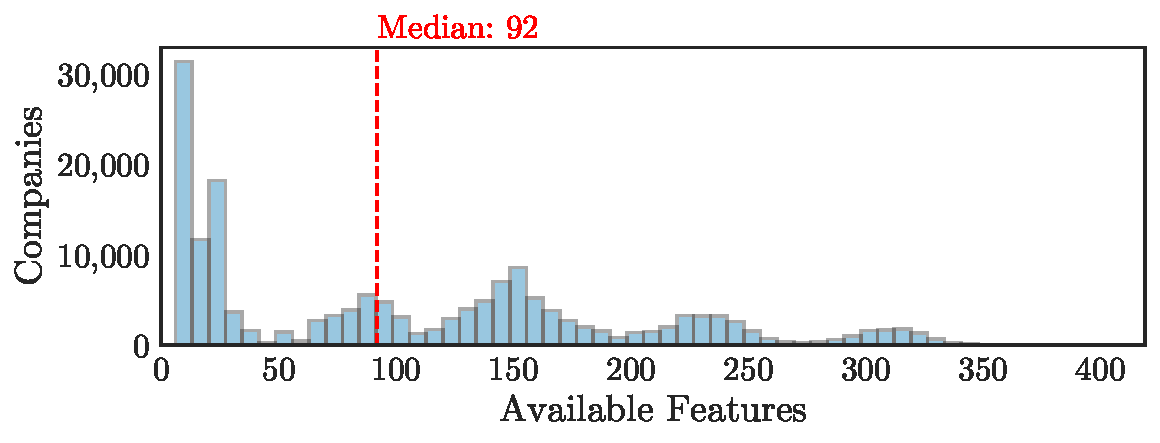
\includegraphics[width=\textwidth]{../figures/design/sparsity_features}
        \caption[Sparsity by company]{Distribution of available features by company.}
        \label{fig:design:sparsity:features}
    \end{subfigure}
    \begin{subfigure}{\textwidth}
        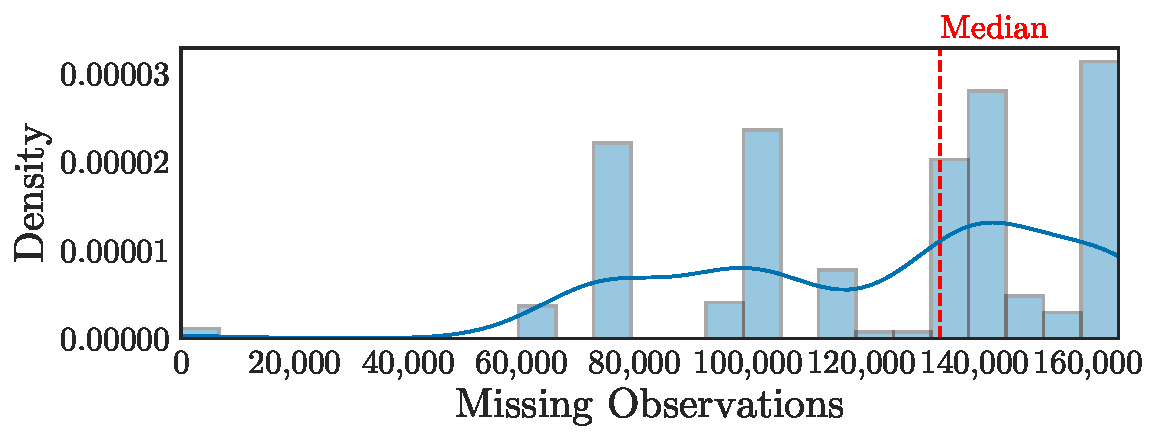
\includegraphics[width=\textwidth]{../figures/design/sparsity_observations}
        \caption[Sparsity by feature]{Distribution of available observations by feature.}
        \label{fig:design:sparsity:observations}
    \end{subfigure}
    \caption[Distribution of sparsity]{Density of features in our dataset.}
    \label{fig:design:sparsity}
\end{figure}

\subsubsection{Normality}

Next, we explored the normality of the dataset. Figure~\ref{fig:design:normality} shows the skewness and kurtosis of the features in our dataset. Skewness is a measure of symmetry, or more precisely, the lack of symmetry. We consider a feature to be highly asymmetrical if its absolute skewness is above 1 and most of our features are more skewed than this cut-off. Kurtosis is a measure of the distribution of variance in a feature. If a feature has high kurtosis we call it `long-tailed'. We use Fisher's measure of kurtosis, which has a normal value of 0. Our kurtosis distribution suggests we have many extreme values (outliers) in our dataset. In combination, these results indicate that most features in our dataset are not normally distributed, but rather are positively-skewed, long-tailed distributions.

\begin{figure}[!htb]
    \centering
    \begin{subfigure}{\textwidth}
        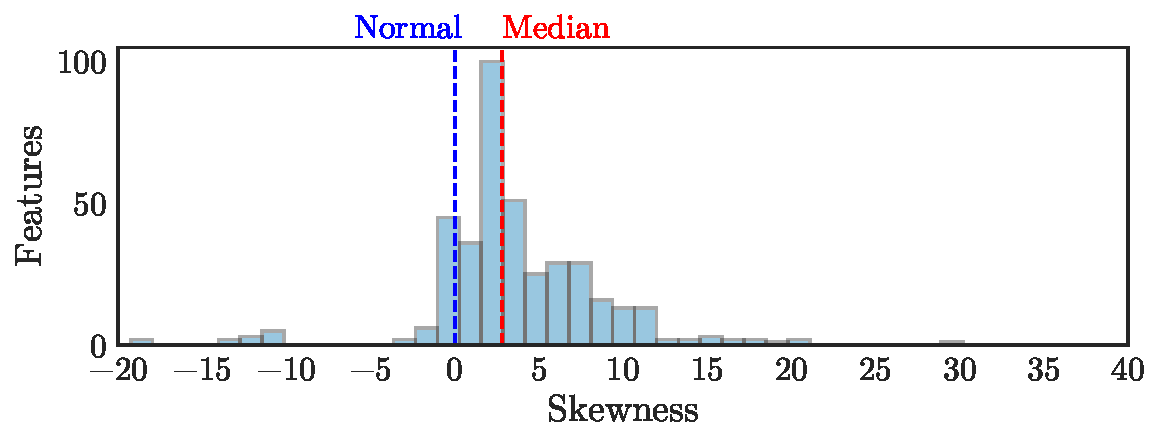
\includegraphics[width=\textwidth]{../figures/design/distribution_skew}
        \caption[Distribution of skewness by feature]{}
        \label{fig:design:normality:skew}
    \end{subfigure}
    \begin{subfigure}{\textwidth}
        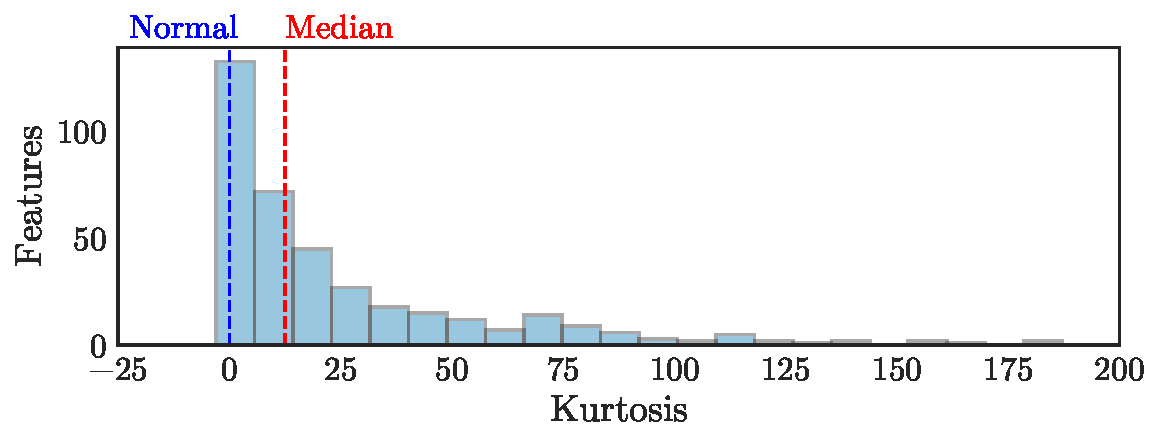
\includegraphics[width=\textwidth]{../figures/design/distribution_kurtosis}
        \caption[Distribution of kurtosis by feature]{}
        \label{fig:design:normality:kurtosis}
    \end{subfigure}
    \caption[Distribution of skewness and kurtosis]{Normality of features in our dataset.}
    \label{fig:design:normality}
\end{figure}

\subsubsection{Scale}

Next, we explored the scaling and range of each of our features. Figure~\ref{fig:design:scaling} shows the \gls{iqr} of each feature. The distribution is extremely skewed in its original domain so we perform a log transformation to make the distribution easier to observe. Even the log-transformed distribution is highly skewed, which shows that our features have a wide range of magnitudes.

\begin{figure}[!htb]
    \centering
    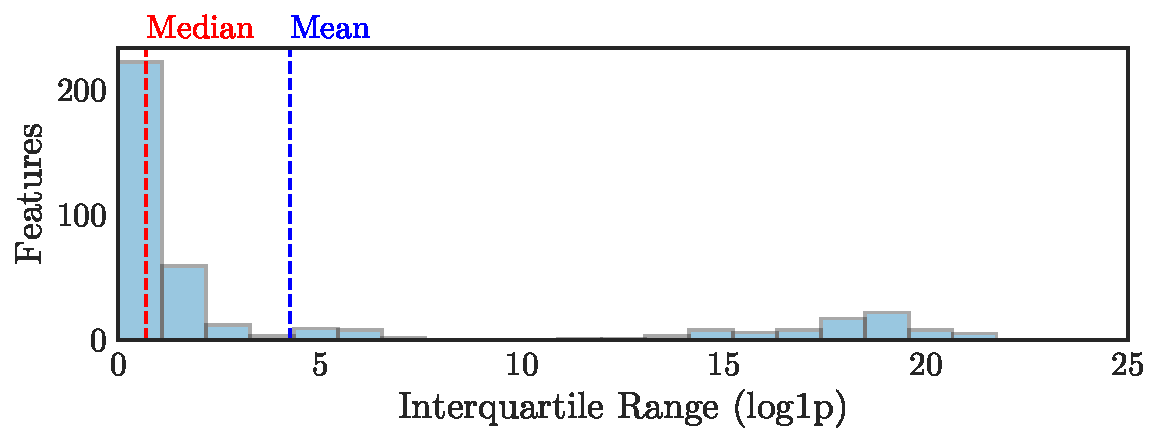
\includegraphics[width=\textwidth]{../figures/design/distribution_ranges}
    \caption[Distribution of interquartile ranges]{Distribution of interquartile ranges (log-transformed) in our dataset.}
    \label{fig:design:scaling}
\end{figure}

\subsubsection{Orthogonality}

Finally, we explored the orthogonality of our features: the extent to which the variance of our features is unrelated. We examined the distribution of pair-wise inter-correlations between our features, as depicted in Figure~\ref{fig:design:orthogonality}. We use two correlation metrics: Pearson and Spearman. Pearson is more commonly used, but Spearman is a ranked metric and may more accurately reflect our non-normal feature distributions~\cite{chok2010}. Although most features have small inter-correlations (\~60\% below 0.2), there are still some that are highly correlated, so it might be efficient to remove these features using unsupervised feature extraction.

\begin{figure}[!htb]
    \centering
    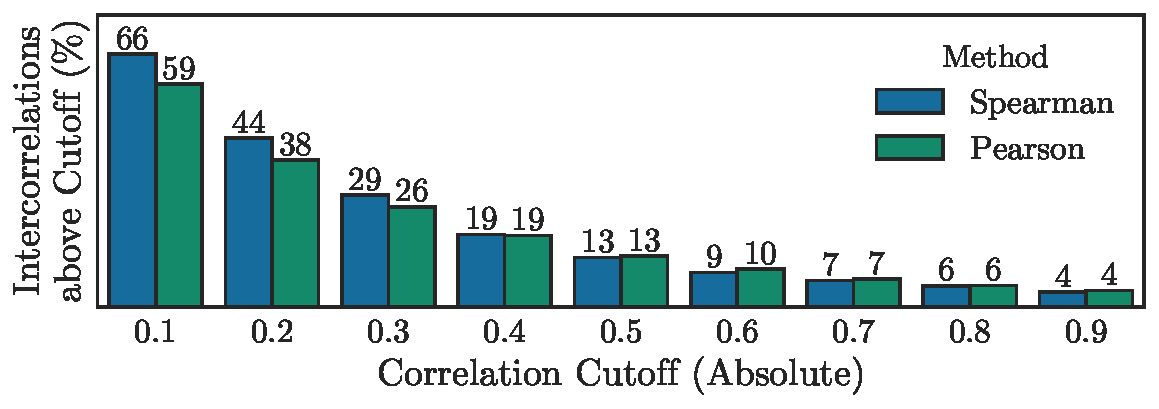
\includegraphics[width=\textwidth]{../figures/design/distribution_orthogonality}
    \caption[Distribution of inter-correlations]{Distribution of inter-correlations in our dataset.}
    \label{fig:design:orthogonality}
\end{figure}

\subsection{Hyperparameter Evaluation}

To address the issues identified in the previous section, we developed a classification pipeline using the popular Python-based machine learning library Scikit-learn~\cite{pedregosa2011}. The classification pipeline construct allows us to search across hyperparameters at each step in the pipeline (e.g. imputation strategy, the number of components extracted in \gls{pca}, see Appendix~\ref{appendix:pipeline_hyperparameters} for the full hyperparameter list). The following section explores the evaluation of the pipeline hyperparameters against an indicative dataset generated from our training database. The indicative dataset is composed of a feature vector from April 2012 and an outcome vector from April 2014.

\subsubsection{Imputation}

After reviewing the distribution of missing data, we decided to investigate imputation methods further. Common imputation strategies include replacing missing values with the mean, median or mode of each feature. Figure~\ref{fig:design:central_tendency} shows the distribution of mean, median and modes for each feature in the dataset. We apply a log-transformation to this figure to make the highly-skewed distribution easier to observe. There is minimal variance between the mean, median and mode of the features. For the majority of features, all three measures of central tendency are equal to zero. This finding resolves the issue of distinguishing missing data from negative observations because, following imputation, all of these data points will map to zero. Figure~\ref{fig:design:imputer} shows the performance of the imputation strategies. All three imputation strategies produce similar results.

\begin{figure}[!htb]
    \centering
    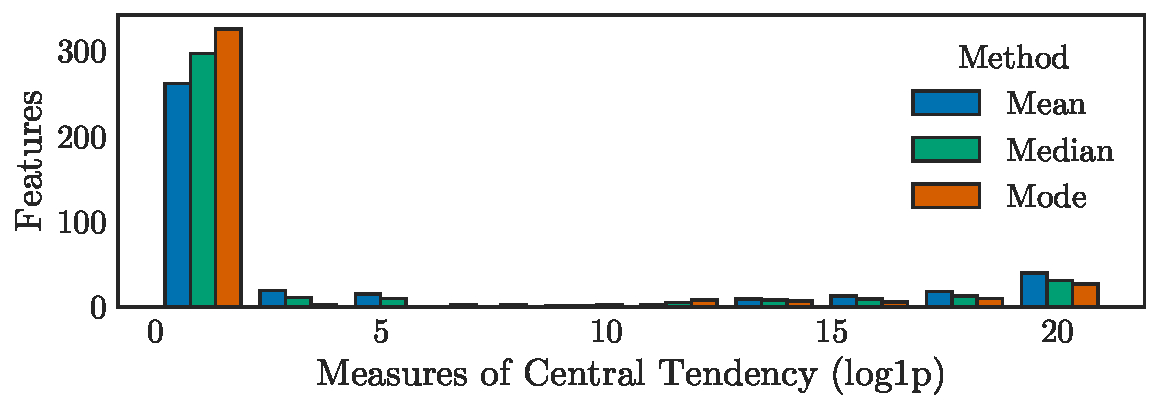
\includegraphics[width=\textwidth]{../figures/design/distribution_central_tendency}
    \caption[Distribution of central tendency]{Distribution of measures of central tendency (mean, median and mode) in our dataset.}
    \label{fig:design:central_tendency}
\end{figure}

\begin{figure}[!htb]
    \centering
    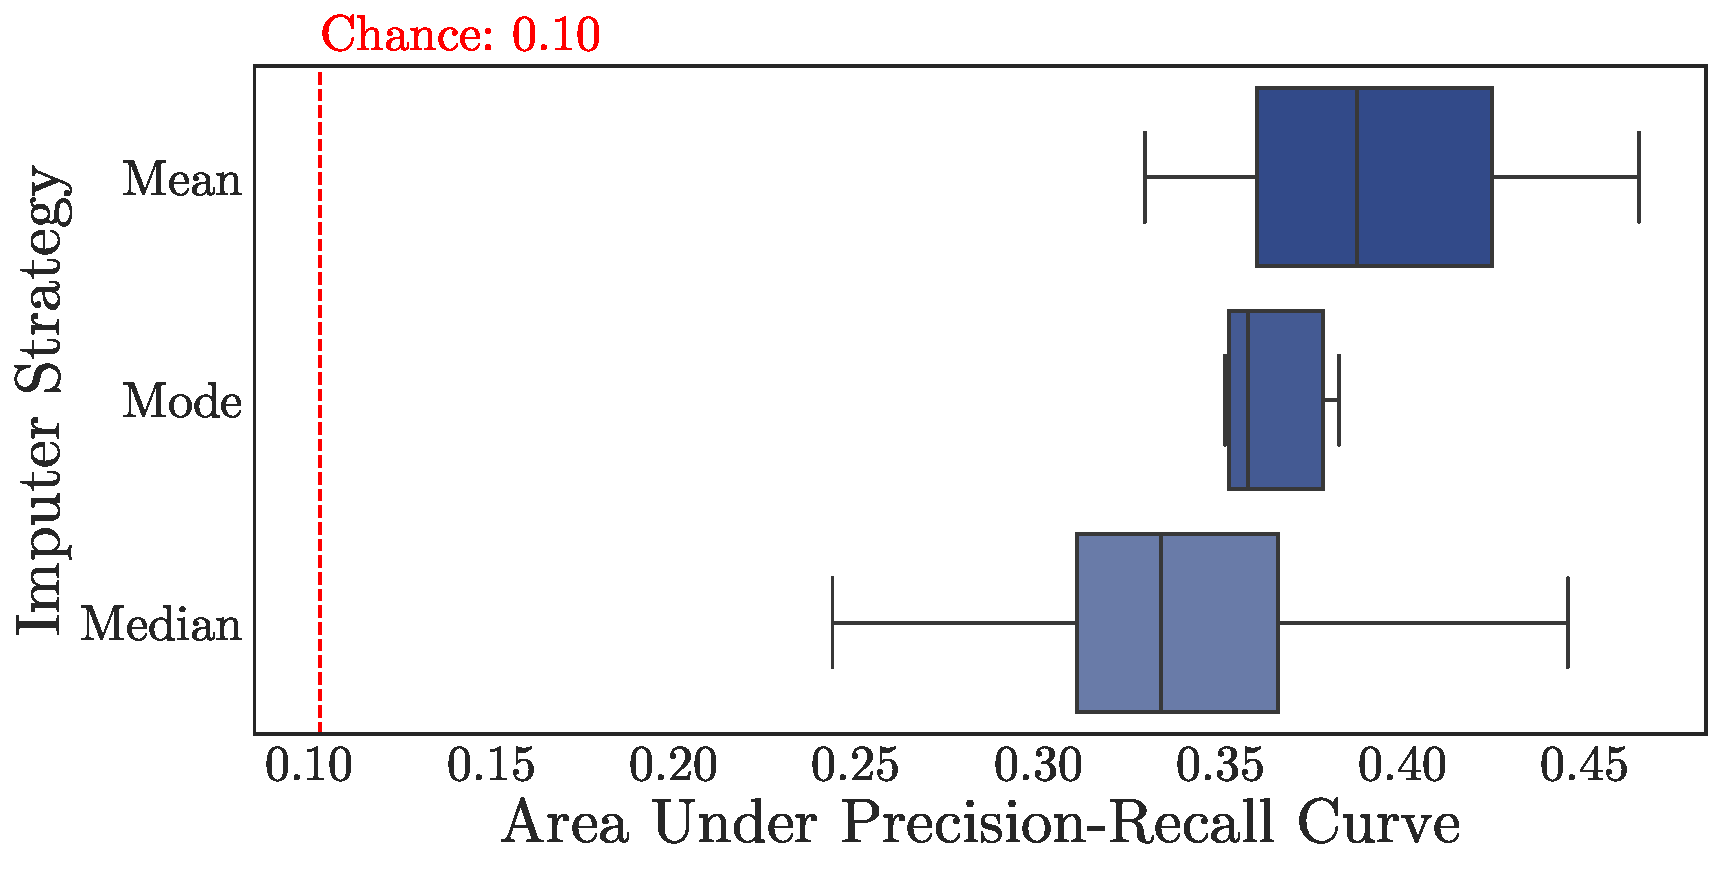
\includegraphics[width=\textwidth]{../figures/design/auc_imputer}
    \caption[Area under \gls{pr} Curves by imputation strategy]{Area under \gls{roc} for different imputation strategies. Imputation strategies include replacing missing values with the most frequent (mode), median and mean value of each respective feature.}
    \label{fig:design:imputer}
\end{figure}

\subsubsection{Transformation}

While the classification algorithms we identified in the previous chapter are robust to violations of normality, it may be beneficial to transform the data if the feature distributions are extreme. Figure~\ref{fig:design:funding_transformation} shows one of the key features, Total Funding Raised, under different transformations. Like many features in our dataset, the distribution of Total Funding Raised is highly skewed. The log transformation reduces this skewness, and square root transformation also reduces this skewness (to a lesser extent). Figure~\ref{fig:design:transformer} shows the performance of these transformation functions. Both functions provide a small improvement, with square root narrowly best.

\begin{figure}[!htb]
    \centering
    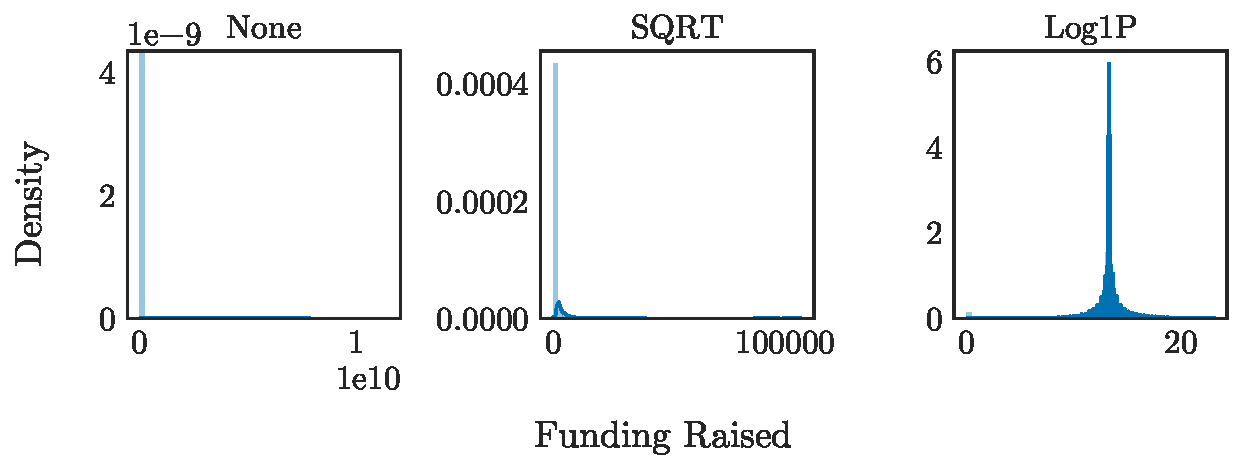
\includegraphics[width=\textwidth]{../figures/design/distribution_funding_transformed}
    \caption[Funding raised transformed by functions]{Funding raised transformed by functions.}
    \label{fig:design:funding_transformation}
\end{figure}

\begin{figure}[!htb]
    \centering
    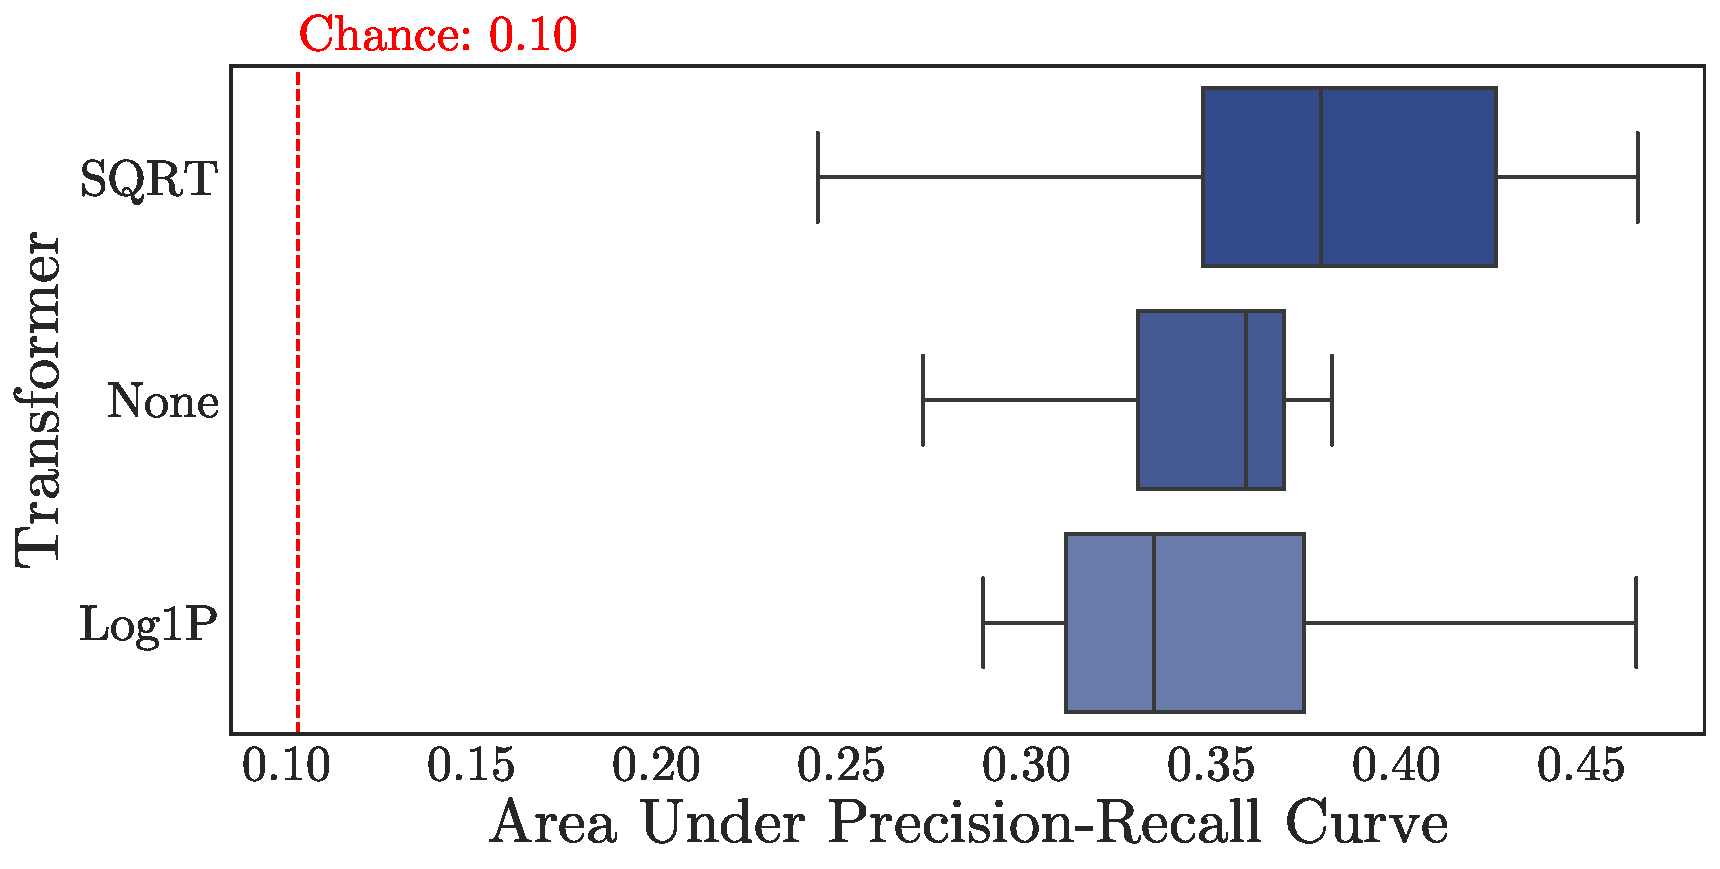
\includegraphics[width=\textwidth]{../figures/design/auc_transformer}
    \caption[Area under \gls{pr} Curves by transformation function]{Area under \gls{roc} for different transformation functions. Transformations include: None (identity transformation), Log1p (natural logarithm of one plus the input array, element-wise), and SQRT (the square root of the input array, element-wise).}
    \label{fig:design:transformer}
\end{figure}

\subsubsection{Scaling}

Standardisation of datasets is a common requirement for many feature extraction methods and machine learning estimators. Scikit-learn provides three primary scaling functions: StandardScaler, RobustScaler and MinMaxScaler. RobustScaler is intended to alleviate the effect of outliers while MinMaxScaler is designed to preserve zero entries in sparse data - both of these are relevant properties for the dataset. Figure~\ref{fig:design:scaler} shows the performance of these scaling functions. No scaling functions outperform the null condition which may be because the transformer already performs some scaling in an earlier step.

\begin{figure}[!htb]
    \centering
    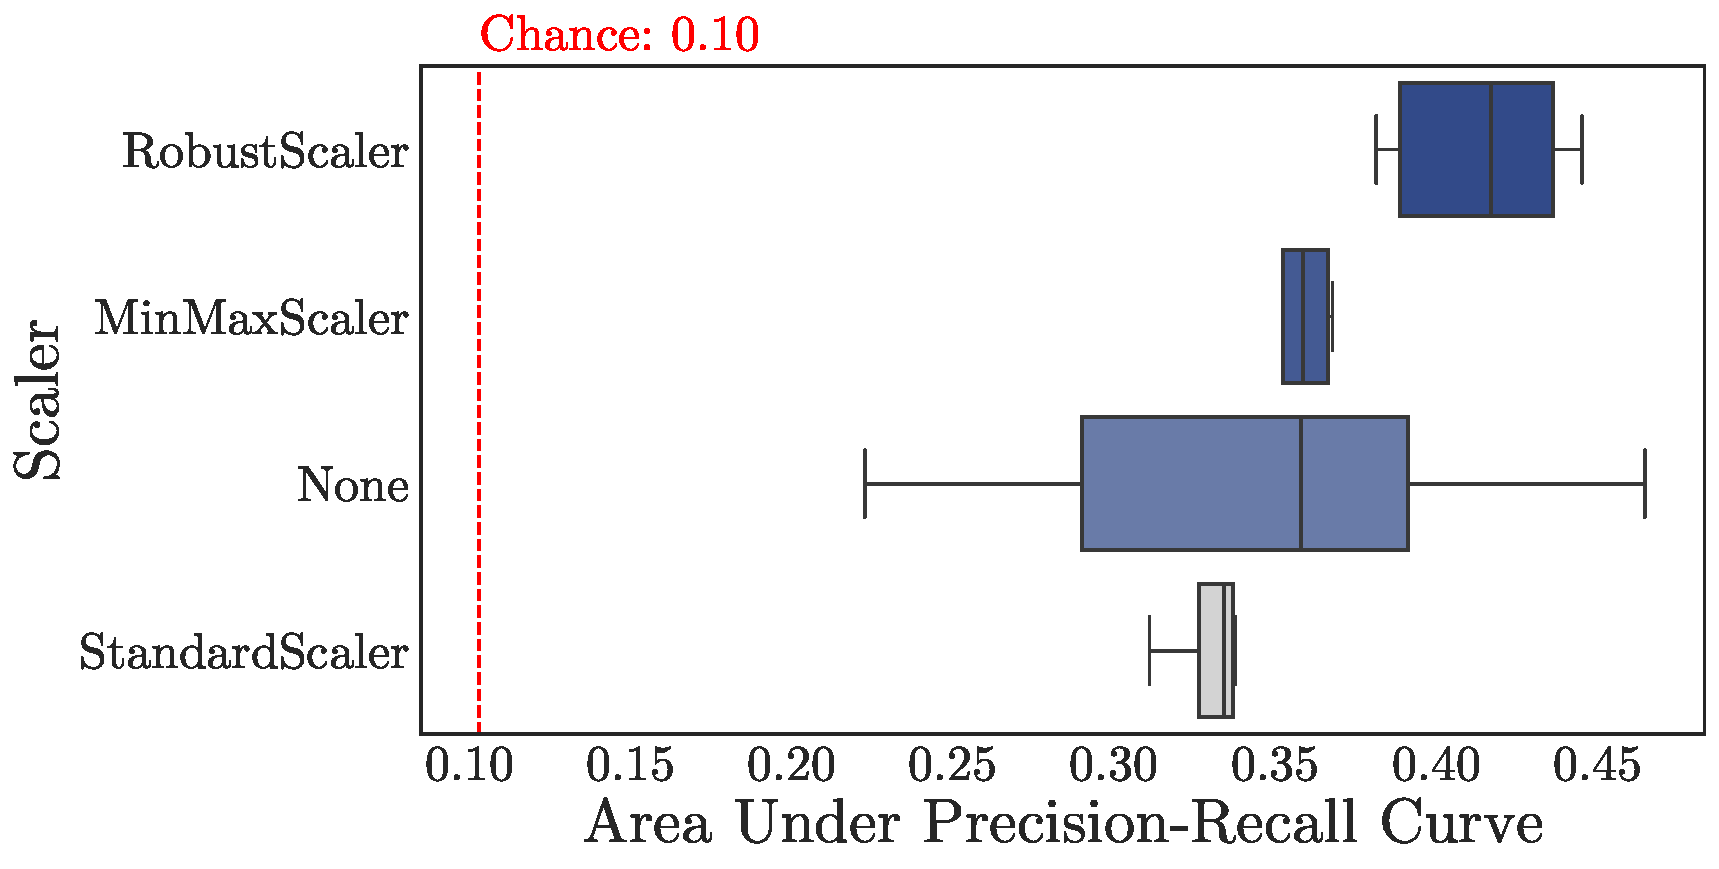
\includegraphics[width=\textwidth]{../figures/design/auc_scaler}
    \caption[Area under \gls{pr} Curves by scaling function]{Area under \gls{roc} for different scaling functions. Scaling functions include: None, StandardScaler (mean: 0, variance: 1), RobustScaler (median: 0, IQR: 1) and MinMaxScaler (min: 0, max: 1).}
    \label{fig:design:scaler}
\end{figure}

\subsubsection{Extraction}

Feature extraction reduces high-dimensional data into lower-dimensional data in such a way that maximises the variance of the data. The most common approach to dimensionality reduction is \gls{pca}. \Gls{pca} is a technique which takes a set of vectors and finds an uncorrelated coordinate system in which to represent these vectors~\cite{friedman2001}. The magnitude of each eigenvector (eigenvalue) is displayed in Figure~\ref{fig:design:scree_plot}. The first ten components capture the majority of explained variance, and the eigenvalues drop below one by 100 components -- this suggests that these are reasonable values for further hyperparameter search. Figure~\ref{fig:design:extractor} shows the \gls{roc} for different numbers of extracted components. All curves produce similar classification results (within the margin of error) which implies that we should extract between 1-20 components because it will provide us with more efficient computation.

\begin{figure}[!htb]
    \centering
    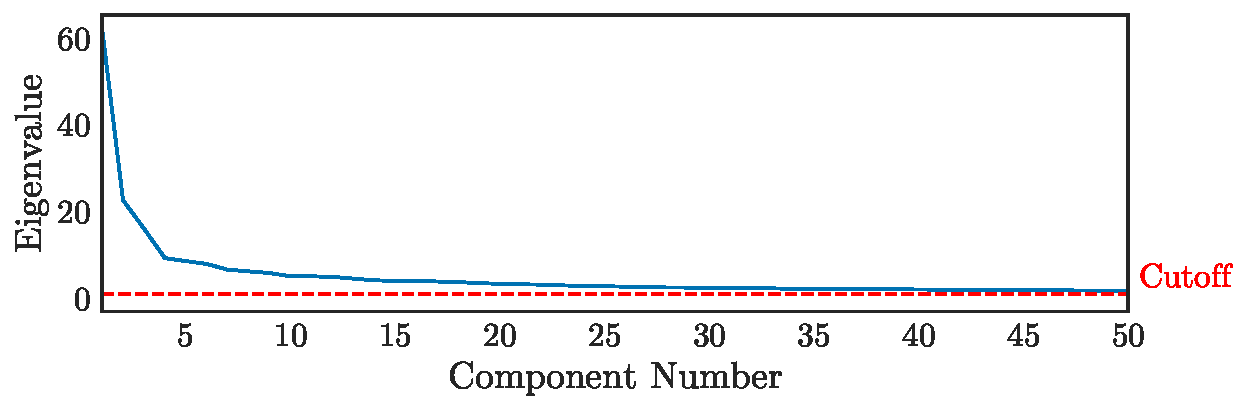
\includegraphics[width=\textwidth]{../figures/design/distribution_eigenvalues}
    \caption[Distribution of eigenvalues -- \gls{pca}]{Eigenvalues extracted from \gls{pca} model. Horizontal line drawn at an Eigenvalue of 1 -- this theoretically represents the `contribution' of one original feature and is commonly used as an approximate threshold for included components.}
    \label{fig:design:scree_plot}
\end{figure}

\begin{figure}[!htb]
    \centering
    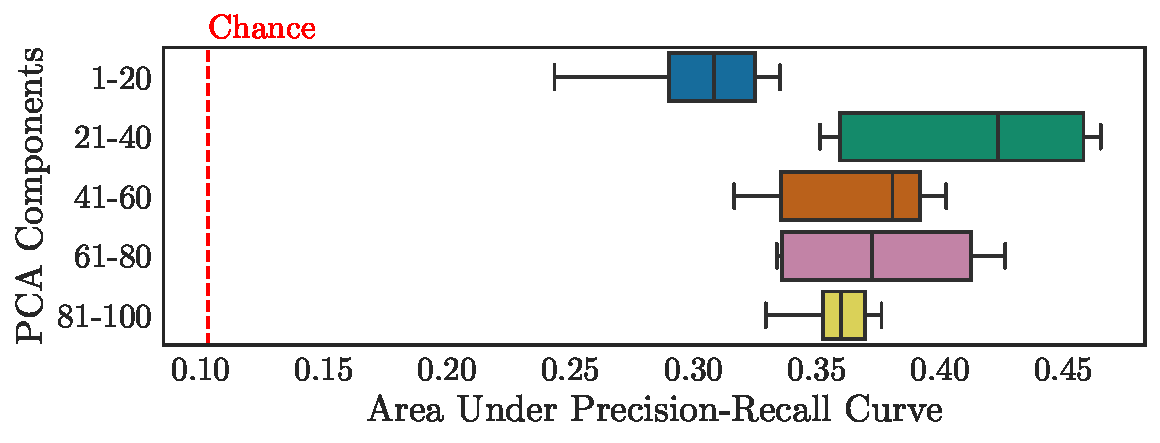
\includegraphics[width=\textwidth]{../figures/design/auc_extractor}
    \caption[Area under \gls{pr} Curves by \gls{pca} techniques]{Area under \gls{roc} for different number of extracted components from \gls{pca}. Curves have been grouped by the quotient of the number of components divided by 20 to result in five ordered groups (e.g. Range [0, 19] becomes 0).}
    \label{fig:design:extractor}
\end{figure}

While \gls{pca} is efficient at reducing features, the resultant components are not interpretable. However, analysis of 400+ individual features is also difficult to interpret. A compromise is to group features using our conceptual framework. We apply an approach that weights each feature to maximise the inter-correlations within each group. We use Spearman Correlation which is more robust than Pearson Correlation to extreme skewness~\cite{chok2010}. Figure~\ref{fig:design:grouped_heatmap} displays the inter-correlations between each grouped factor. Overall, there is little correlation between these grouped factors. This finding is promising because it implies that each group provides unique information. There are some minor correlations: Advisors are somewhat correlated with Founders and Investors, and Economic factors are somewhat correlated with Executives and Funding factors.

\begin{figure}[!htb]
    \centering
    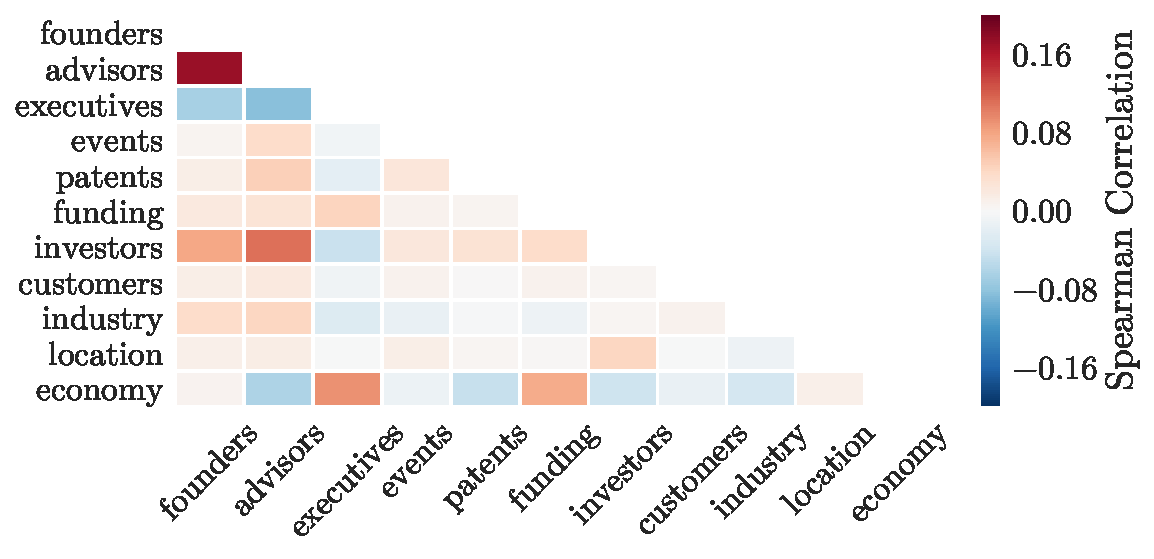
\includegraphics[width=\textwidth]{../figures/design/distribution_correlations_grouped}
    \caption[Inter-correlations of factors from framework]{Inter-correlations of each factor from conceptual framework. Spearman ranking correlation is used. Individual features are grouped by applying weights that maximise the inter-correlations within each group from our conceptual framework (see Figure~\ref{fig:design:features:framework_details}).}
    \label{fig:design:grouped_heatmap}
\end{figure}

\subsubsection{Classification Algorithms}

The literature review we performed in the previous chapter identified common supervised classification algorithms potentially suitable for application to \gls{vc} investment screening. Our analysis suggested that Random Forests were most likely to provide an optimal trade-off between predictive power, interpretability and time taken. We empirically tested each of these classifiers and compared their performance against a range of metrics, as displayed in Table~\ref{fig:design:classification_metrics}. We report maximum and median scores so as not to penalise algorithms that have unfavourable hyperparameter search spaces.

\begin{table}[!htb]
    \centering
    \scalebox{0.8}{\begin{tabular}{lrrrrrrrrrr}
\toprule
{} & \multicolumn{2}{c}{AUC PRC}        & \multicolumn{2}{c}{AUC ROC}        &     \multicolumn{2}{c}{F1}       &    \multicolumn{2}{c}{MCC}        & \multicolumn{2}{c}{Fit Time (s)}         \\
{Classifier} &    Median &    Max &    Median &    Max &   Median &    Max &   Median &    Max &         Median &     75th \\
\midrule
LR       &   0.417 &  0.465 &   0.675 &  0.710 &  0.339 &  0.358 &  0.255 &  0.288 &        7.3 &  412.7 \\
RF             &   0.376 &  0.465 &   0.619 &  0.709 &  0.332 &  0.360 &  0.271 &  0.288 &       68.3 &   69.0 \\
DT             &   0.388 &  0.429 &   0.651 &  0.659 &  0.305 &  0.314 &  0.212 &  0.224 &       15.3 &   16.8 \\
NB               &   0.354 &  0.367 &   0.623 &  0.638 &  0.303 &  0.321 &  0.212 &  0.239 &        8.6 &   26.8 \\
KNN       &   0.335 &  0.353 &   0.532 &  0.565 &  0.131 &  0.226 &  0.137 &  0.210 &        8.5 &   20.8 \\
ANN &   0.320 &  0.335 &   0.517 &  0.523 &  0.072 &  0.096 &  0.111 &  0.140 &        9.1 &   21.0 \\
SVM    &   0.233 &  0.244 &   0.503 &  0.504 &  0.014 &  0.017 &  0.038 &  0.045 &       29.0 &   29.0 \\
Total                     &   0.357 &  0.465 &   0.623 &  0.710 &  0.300 &  0.360 &  0.209 &  0.288 &       15.3 &   29.0 \\
\bottomrule
\end{tabular}
}
    \caption[Overview of classification algorithm performance]{Overview of classification algorithm performance. Algorithms are: NB~=~Naive Bayes, LR~=~Logistic Regression, KNN~=~K-Nearest Neighbours, DT~=~Decision Trees, RF~=~Random Forests, SVM~=~Support Vector Machines, ANN~=~Artificial Neural Networks.}
    \label{fig:design:classification_metrics}
\end{table}

We take a closer look at the \gls{pr} curves for each classifier in Figure~\ref{fig:design:classifier}. While all classifiers perform better than chance, Logistic Regressions and Random Forests come out ahead, and Support Vector Machines and Artificial Neural Networks appear to underperform. Examining the cross-validated learning curves for each classifier (Figure~\ref{fig:design:create_learning_curves}), we see that Naive Bayes, Logistic Regression, Artificial Neural Networks and Support Vector Machines quickly converge, whereas Decision Trees, Random Forests and K-Nearest Neighbours require more observations to converge. This suggests that Random Forests may do better in final testing (which will not be cross-validated) and in the future as the dataset grows.

\begin{figure}[!htb]
    \centering
    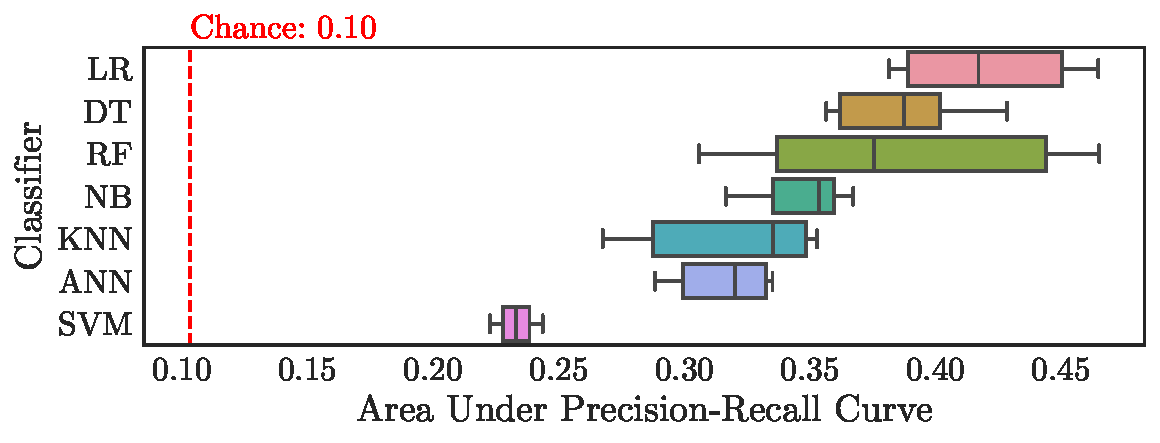
\includegraphics[width=\textwidth]{../figures/design/auc_classifier}
    \caption[Area under \gls{pr} Curves by classification algorithms]{Area under \gls{roc} for different classification algorithms. All algorithms are implementations from the Sci-kit learn library. Algorithms are: NB~=~Naive Bayes, LR~=~Logistic Regression, KNN~=~K-Nearest Neighbours, DT~=~Decision Trees, RF~=~Random Forests, SVM~=~Support Vector Machines, ANN~=~Artificial Neural Networks.}
    \label{fig:design:classifier}
\end{figure}

\begin{figure}[!htb]
    \centering
    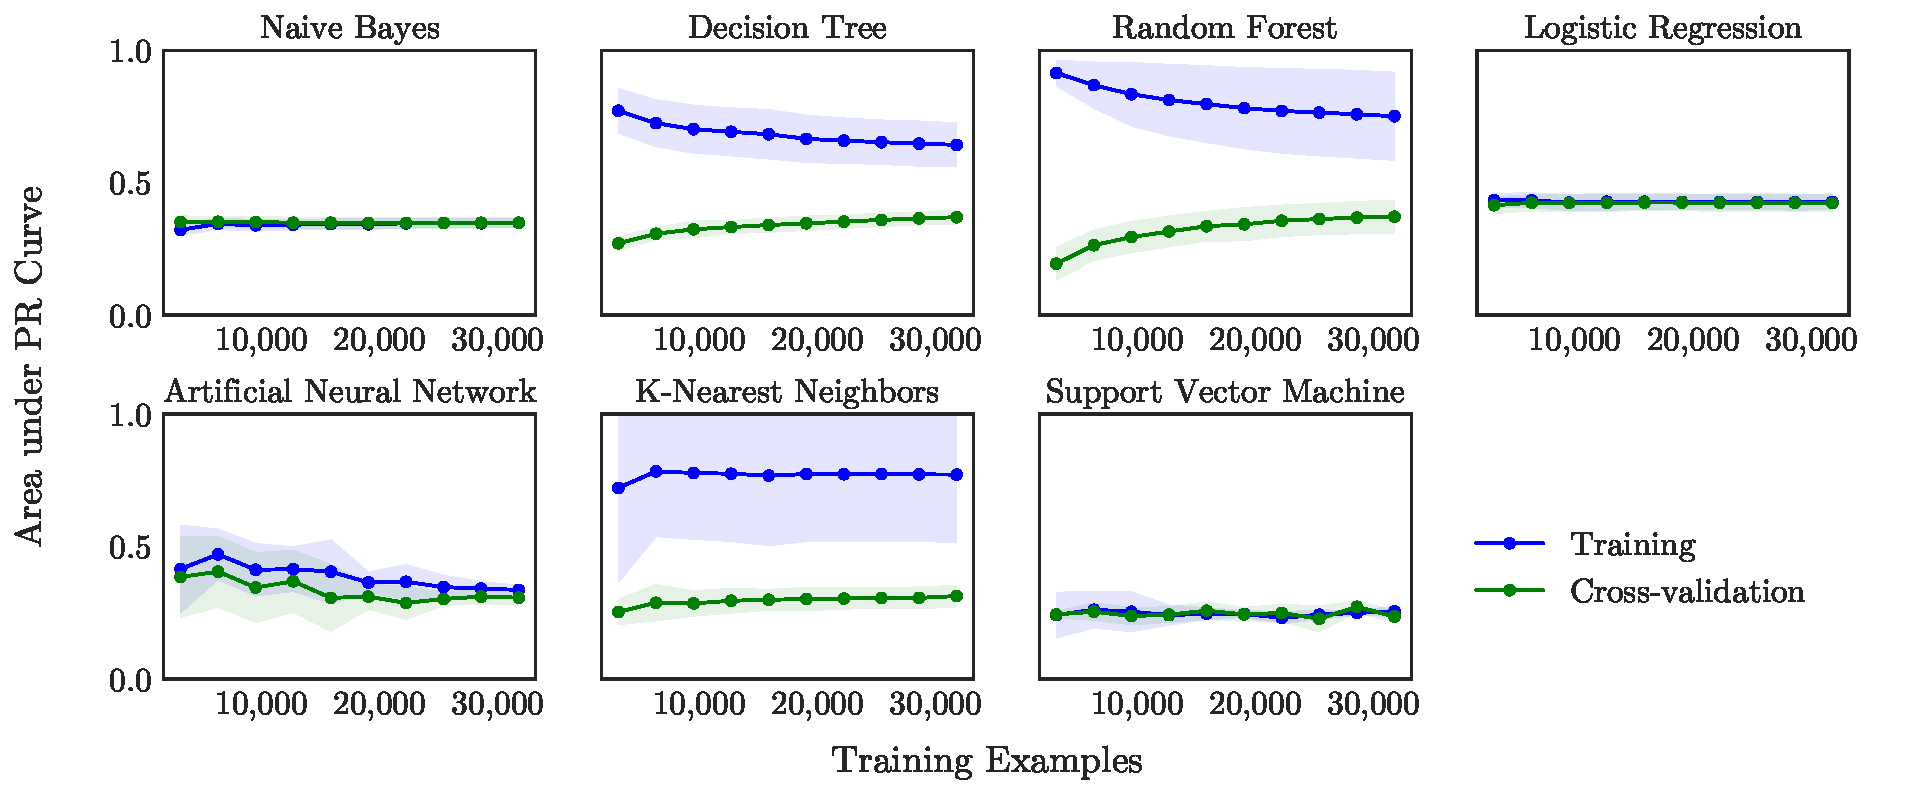
\includegraphics[width=\textwidth]{../figures/design/learning_curves_classifier}
    \caption[Learning curves by classification algorithms]{Learning curves by classification algorithms.}
    \label{fig:design:create_learning_curves}
\end{figure}

\section{Pipeline Selection}

In this step, we evaluate the best pipelines from the previous step over different dataset slices. This process, depicted in Figure~\ref{fig:design:pipeline_selection}, ensures our final pipeline is robust in its performance over time. We aggregate the results for each finalist pipeline across these dataset slices and rank the finalist pipelines on their overall performance. Finally, we select the best pipeline.

\begin{figure}[!htb]
    \centering
    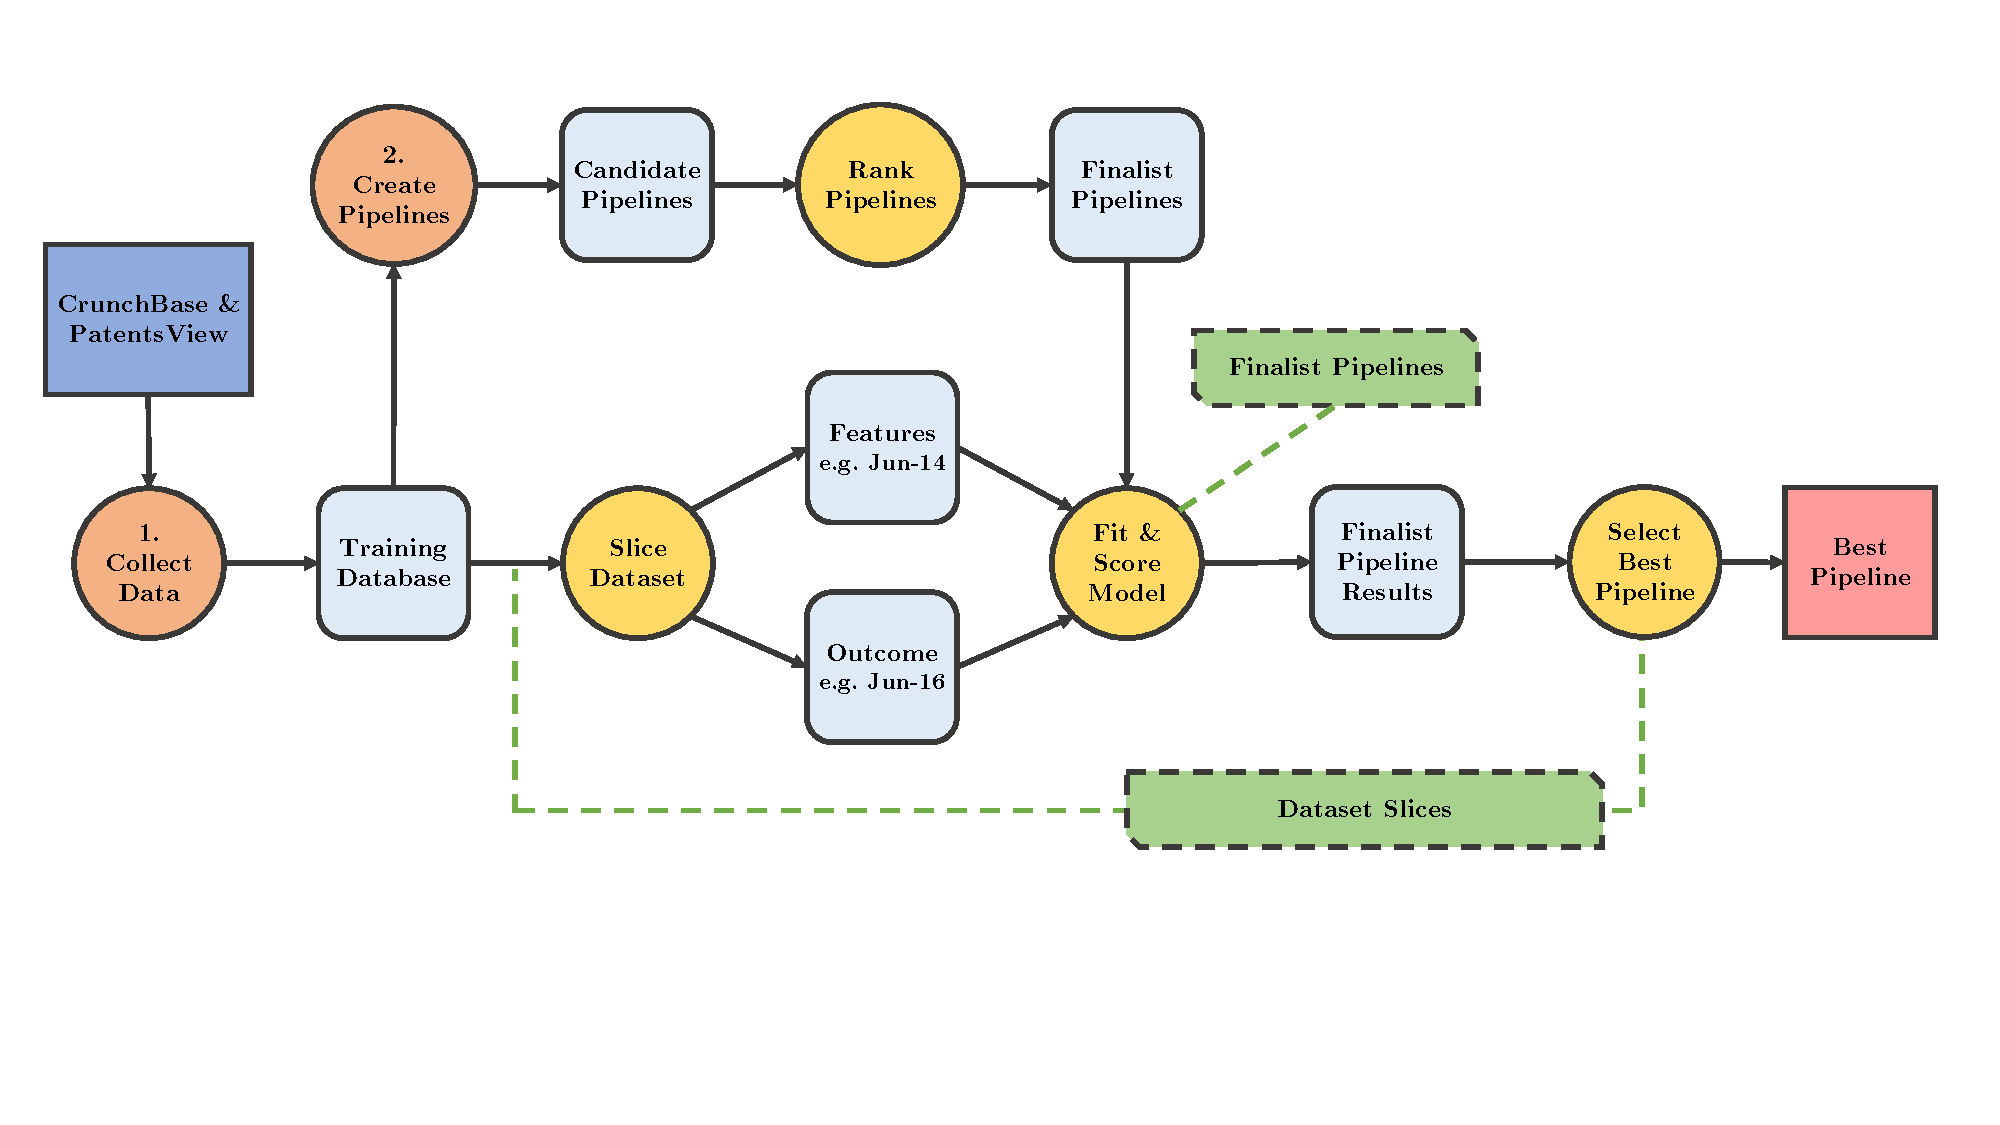
\includegraphics[width=\textwidth]{../figures/design/flowchart_pipeline_selection}
    \caption[Pipeline selection flowchart]{Pipeline selection overview. Legend: dark blue square~=~input, orange circle~=~system component, yellow circle~=~process, light blue rounded square~=~intermediate, red square~=~output, green hexagon: iterative process / search space.}
    \label{fig:design:pipeline_selection}
\end{figure}

\subsection{Evaluation Metrics}

Next, we decided how to select finalist pipelines that we can evaluate further. There are a variety of metrics used to assess binary classification algorithms. Accuracy is rarely used in practice because it gives misleading results in the case of imbalanced classes. \Gls{roc} curves are commonly used, which show how the number of correctly classified positive examples varies with the number of incorrectly classified negative examples. The area under these curves gives a standardised result across a spectrum of decision thresholds. \Gls{pr} curves are similar to \gls{roc} curves but instead map the trade-offs between precision and recall. They are less commonly used than \gls{roc} curves but have been shown to produce more accurate results for imbalanced classes than \gls{roc} curves~\cite{davis2006}. We decided to proceed with \gls{pr} curves because our dataset is highly imbalanced. We will also use this metric to rank our finalist pipelines.

\subsection{Finalist Pipeline Evaluation}

Our hypothesis is that the performance of our pipelines may vary with respect to the dates of our datasets. To evaluate this hypothesis, first, we explored variance between the pipelines on aggregate against the slice dates, presented in Figure~\ref{fig:design:selection_agg_slice}. There is no relationship observed between slice date and score.

\begin{figure}[!htb]
    \centering
    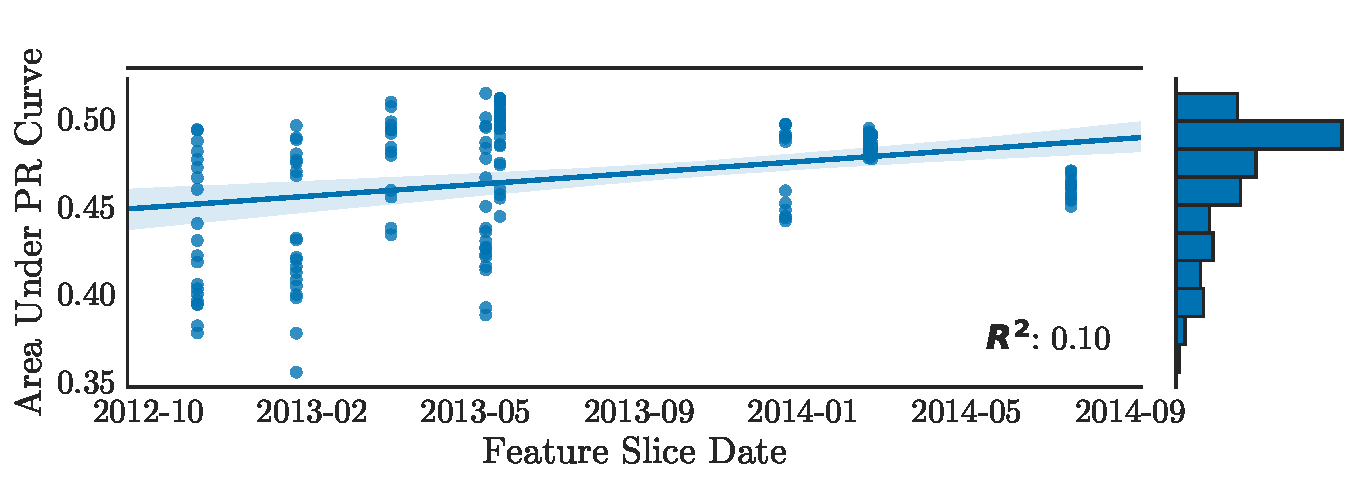
\includegraphics[width=\textwidth]{../figures/design/auc_finalists_agg}
    \caption[Pipeline performance by slice date]{Pipeline performance by slice date.}
    \label{fig:design:selection_agg_slice}
\end{figure}

Next, we study the variance within the individual pipelines, presented in Figure~\ref{fig:design:selection_agg_rank}. Although there is a positive correlation between the pipelines initial ranking and their scores, there are deviations. For example, the top-ranked pipeline from the first stage has a lower median score than the second-ranked pipeline. These results suggest that the top 3-5 pipelines should be evaluated in this manner to ensure that the best pipeline is selected. We describe the chosen pipeline in Table~\ref{appendix:experimental_config}. We adopted this pipeline for our following experiments.

\begin{figure}[!htb]
    \centering
    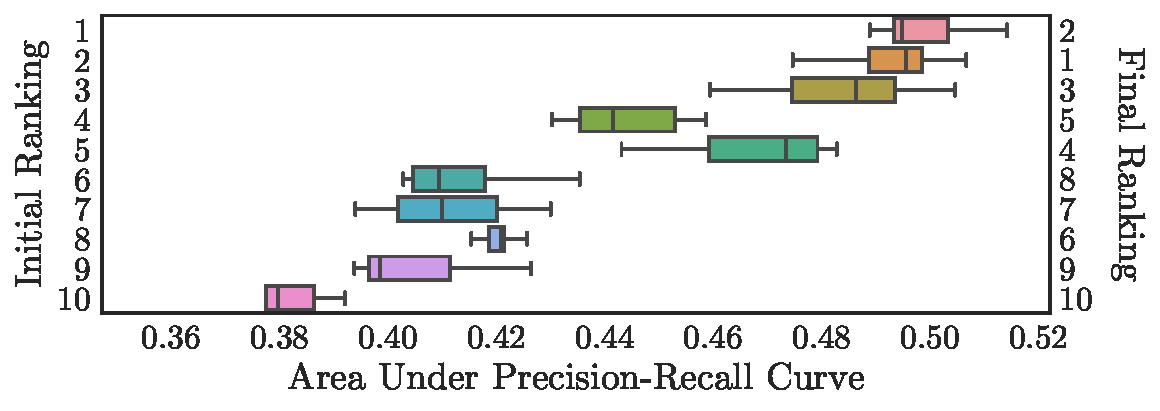
\includegraphics[width=\textwidth]{../figures/design/auc_finalists_rank}
    \caption[Overview of finalist pipeline performance]{Overview of finalist pipeline performance.}
    \label{fig:design:selection_agg_rank}
\end{figure}

\section{Model Fit and Prediction}

Finally, our system applies the best classification pipeline to a feature vector from a held-out test database to generate a model and a set of predictions, as shown in Figure~\ref{fig:design:make_predictions}. We evaluate the accuracy of the models produced by our system in the next chapter.

\begin{figure}[!htb]
    \centering
    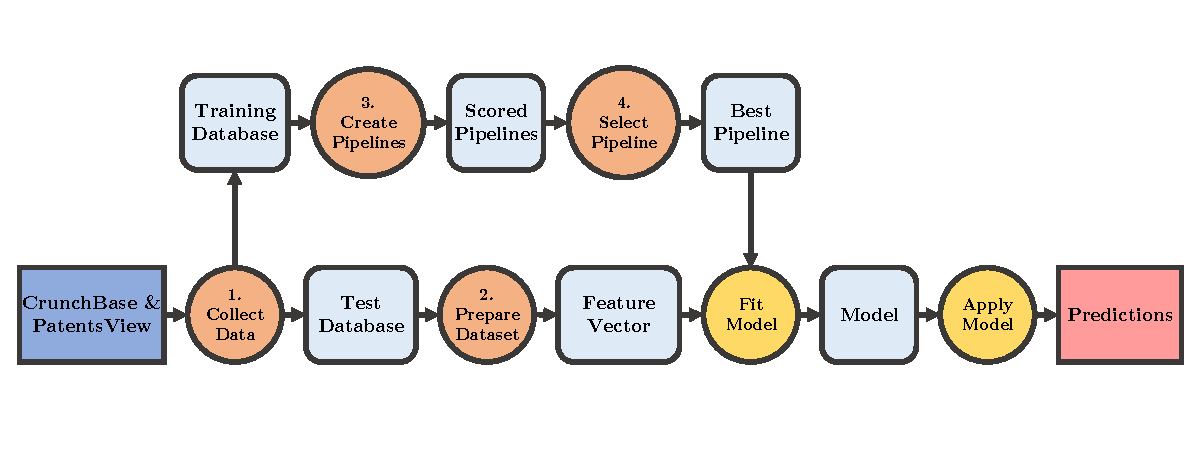
\includegraphics[width=\textwidth]{../figures/design/flowchart_make_predictions}
    \caption[Model fit and prediction flowchart]{Model fit and prediction overview. Legend: dark blue square~=~input, orange circle~=~system component, yellow circle~=~process, light blue rounded square~=~intermediate, red square~=~output.}
    \label{fig:design:make_predictions}
\end{figure}

\ifcsdef{mainfile}{}{\printbibliography}
\end{document}
